% \documentclass[11pt]{scrartcl}
\documentclass[11pt]{article}
\usepackage[sexy]{evan}
\usepackage{graphicx}
\usepackage{answers}
\usepackage{amsmath, amssymb}
\usepackage{hyperref}
\usepackage{mathtools}
\usepackage{multirow}
\usepackage{float}
\usepackage{caption}
\usepackage{subcaption}
\usepackage{pifont}
\usepackage{chngcntr}
\usepackage{footnote}
\usepackage{tikz}
\usetikzlibrary{shapes.geometric, arrows}

\tikzstyle{startstop} = [rectangle, rounded corners, minimum width = 2cm, minimum height=1cm,text centered, draw = black]
\tikzstyle{io} = [trapezium, trapezium left angle=70, trapezium right angle=110, minimum width=2cm, minimum height=1cm, text centered, draw=black]
\tikzstyle{process} = [rectangle, minimum width=3cm, minimum height=1cm, text centered, draw=black]
\tikzstyle{decision} = [diamond, aspect = 3, text centered, draw=black]
\tikzstyle{arrow} = [->,>=stealth]


\counterwithin{figure}{section}
\numberwithin{equation}{section}
\Newassociation{hint}{hintitem}{all-hints}
\renewcommand{\solutionextension}{out}
\renewenvironment{hintitem}[1]{\item[\bfseries #1.]}{}
\declaretheorem[style=thmbluebox,name={Theorem}]{thm}
\setlength{\parindent}{0pt}

\newenvironment{solution}
  {\renewcommand\qedsymbol{$\blacksquare$}\begin{proof}[Solution]}
  {\end{proof}}

\begin{document}
\title{INDENG 262A}
\author{Fengzhe Shi}
\thispagestyle{empty}
$ $
\vfill
\begin{center}

\centerline{\huge \textbf{INDENG 262A Notes, Fall 2020}}
\centerline{\Large \textbf{Mathimatical Programming} } 
\centerline{Professor: Alper Atamt\"{u}rk}
\centerline{Fengzhe Shi}
\end{center}
\vfill
$ $
\newpage
\thispagestyle{empty}
\tableofcontents
\newpage
%\maketitle
\section{Week 1 Lecture}
\subsection{Optimization Problem}
An optimization problem ($P$) has the following format,
\begin{align*}
    \max /\min\ &f(x)\\
    \st \ &g_i(x)\leq b_i, \ i=1,\cdots,m\\
    & x\in S \subseteq \mathbb{R}^n \\
\end{align*}
$F= \left\{ x\in S:\ g_i(x)\leq b_i, \ i=1,\cdots,m \right\} $

\subsection{Feasible Region/Sets}
$x\in F$ is called feasible point.
\begin{definition}
    If $F\neq \phi$, then $P$ is infeasible.
\end{definition}
\begin{definition}
    If $\exists x \in F \ s.t.\ f(x)\geq \lambda$, $\forall \lambda \in \mathbb{R}$, then $P$ is unbounded.
\end{definition}
\begin{definition}
    $\bar{x}\in F$ is a global maximizer of $P$ if $f(\bar{x})\geq f(x), \ \forall x \in F$.
\end{definition}

\begin{example}
    Show that $$\max \{ f(x):x \in F \}=-\min \{ f(x):x\in F \}$$
\end{example}

\subsection{Definitions}
\begin{definition}
    Let $x\in \mathbb{R}^n, \ 0<\epsilon \in R$, the epsilon neighborhood of $x$ in $\mathbb{R}^n$ is the set $N_\epsilon (x)=\{ y\in \mathbb{R}^n:||x-y||\leq \epsilon \}$.
\end{definition}
\begin{definition}
    $S \subseteq \mathbb{R}^n$ is \underline{\textit{bounded}} if $S \subseteq N_\epsilon(0)$ for some $\epsilon >0$.
\end{definition}
\begin{definition}
    $x\in S \subseteq \mathbb{R}^n$ is an \textit{\underline{interior point}} of $S$ if $N_\epsilon(x) \subset S$ for some $\epsilon >0$.
\end{definition}
\begin{definition}
    $x\in S \subseteq \mathbb{R}^n$ is a \underline{\textit{boundary point}} if $N_\epsilon(x) \subset S$ contains at least one point in $S$ and at least one point not in $S$ for any $\epsilon >0$.
\end{definition}
\begin{definition}
    Closure of $S \subseteq \mathbb{R}^n$ is the set $cl(S) \subset S \cup bd(S)$.
\end{definition}
\begin{definition}
    $S$ is closed if $S=cl(S)$.
\end{definition}
\begin{definition}
    $S$ is open if $S=int(S)$.
\end{definition}

\begin{example}
    Let $S=\{ (x,y)\in \mathbb{R}^2:\ x^2+y^2 \leq 1 \}$, \begin{align*}
        &int(S)=\{ (x,y)\in \mathbb{R}^2:\ x^2+y^2 < 1 \} \\
        &bd(S)=\{ (x,y)\in \mathbb{R}^2:\ x^2+y^2 = 1 \}
    \end{align*}
    $\mathbb{R}^2$, $\phi$ are both open and closed.
\end{example}

\begin{definition}
    $\bar{x}\in F$ is called a \underline{\textit{local minimizer}} if there exists small $\epsilon>0 \ \st \ f(\bar{x})\leq f(x) \quad \forall x \in F:\ x\in N_\epsilon(\bar{x})$
\end{definition}

\begin{figure}[H]
    \centering
    \includegraphics[width=10cm]{images/1-ex-1.png}
    \caption{Some local minimizers $a$, $\left[ b,c \right]$, $e$ and global minimizers $\left[ b,c \right]$}
\end{figure}

Non-existence of optima:
\begin{enumerate}[1)]
    \item $F=\phi$
    \item $F=R_+$, $F$ unbounded
    \item $F=(a,b)$, $F$ not closed
    \item $F=[a,b]$, $f$ not continuous
\end{enumerate}

\begin{theorem}[Weierstrass Theorem]\label{eqn:Weierstrass}
    Let $F$ be a nonempty compact (bounded, closed) set, and $f:F\rightarrow \mathbb{R}$ be continuous on $F$. Then $\min\{ f(x):x\in F \}$ attains its minimum (there exists minimizer in $F$).
    \begin{proof}
        $f$ continuous, $F$ bounded, closed, $F\neq \phi$, $\exists \alpha \equiv inf\{f(x):x\in F\}$
    \end{proof}
\end{theorem}

\begin{definition}
    $\alpha$ is the greatest lower bound in $f$ on $F$: $\alpha \leq f(x), \ \forall x \in F$ and $\nexists \bar{\alpha}>\alpha\ s.t.\ \bar{\alpha}\leq f(x), \ \forall x \in F$.
\end{definition}

\subsection{Combinations}
Let $x^i$ be vectors in $\RR^n$, $i=1, \cdots, k$.
\begin{definition}
    $\bar{x} \in \RR^n$ is a \underline{\textit{convex combination}} of $\left\{ x^i \right\}$, if $\bar{x}=\sum_{i=1}^k \lambda_i x^i$ subject to $\sum_{i=1}^k \lambda_i=1, \ \lambda \geq 0$.
\end{definition}
\begin{definition}
    $\bar{x} \in \RR^n$ is a \underline{\textit{conic combination}} of $\left\{ x^i \right\}$, if $\bar{x}=\sum_{i=1}^k \lambda_i x^i, \ \lambda \geq 0$.
\end{definition}
\begin{definition}
    The \underline{\textit{convex hull}} of $\left\{ x^i \right\}$ is the set of all convex combinations of the vectors.
\end{definition}

\begin{figure}[H]
    \centering
    \begin{minipage}{.5\textwidth}
      \centering
      \includegraphics[width=.3\linewidth]{images/1-ex-2.png}
      \captionof{figure}{Convex combinations}
    \end{minipage}%
    \begin{minipage}{.5\textwidth}
      \centering
      \includegraphics[width=.3\linewidth]{images/1-ex-3.png}
      \captionof{figure}{Conic combination}
    \end{minipage}
\end{figure}

\newpage
\section{Week 2 Lecture}
\subsection{Convexity}
\begin{definition}
    $S \subseteq \mathbb{R}^n$ is convex if $\lambda x^1 + (1-\lambda)x^2 \in S, \ \forall x^1,x^2\in S, \ \lambda\in [0,1]$.
\end{definition}

\begin{figure}[H]
    \centering
    \begin{minipage}{.5\textwidth}
      \centering
      \includegraphics[width=.3\linewidth]{images/2-ex-1.png}
      \captionof{figure}{Convex}
    \end{minipage}%
    \begin{minipage}{.5\textwidth}
      \centering
      \includegraphics[width=.3\linewidth]{images/2-ex-2.png}
      \captionof{figure}{Not convex}
    \end{minipage}
\end{figure}

\begin{definition}
    Let $S \subseteq \mathbb{R}^n$ be a convex set. Let $f:\mathbb{R}^n\rightarrow \mathbb{R}$.
    \begin{enumerate}[(i)]
        \item $f$ is a convex function on $S$ if \begin{align*}
            f(\lambda x^1 + (1-\lambda)x^2) \leq \lambda f(x^1) + (1-\lambda)f(x^2), \ \forall x^1,x^2\in S, \ \lambda\in [0,1]
        \end{align*}
        \item $f$ is strictly convex on $S$ if \begin{align*}
            f(\lambda x^1 + (1-\lambda)x^2) < \lambda f(x^1) + (1-\lambda)f(x^2), \ \forall x^1,x^2\in S, \ \lambda\in (0,1)
        \end{align*}
    \end{enumerate}
\end{definition}

\begin{figure}[h]
    \centering
    \includegraphics[scale = 0.5]{images/2-ex-3.png}
    \caption{A convex function}
\end{figure}

\begin{definition}
    Let $S \subseteq \mathbb{R}^n$ be a convex set. $f:\mathbb{R}^n\rightarrow \mathbb{R}$ is concave on $S$ if $f(\lambda x^1 + (1-\lambda)x^2) \geq \lambda f(x^1) + (1-\lambda)f(x^2), \ \forall x^1,x^2\in S, \ \lambda\in [0,1]$.
\end{definition}

\textbf{Remark}: $f$ is convex if and only if $-f$ is concave. 

\begin{definition}
    $f:\mathbb{R}^n\rightarrow \mathbb{R}$ is an affine function if $f(x)=\sum^n_{j=1}a_jx_j+a_0,\ a_j \in \mathbb{R}$. If $a_0=0$, then $f$ is linear.
\end{definition}
\begin{definition}
    Epigraph of function $f:\mathbb{R}^n\rightarrow \mathbb{R}$ is \begin{align*}
        \operatorname{epi}(f)=\{(x,y)\in \mathbb{R}^{n+1}:f(x)\leq y\}
    \end{align*}
\end{definition}

\begin{definition}
    Hypograph of function $f$ is \begin{align*}
        \operatorname{hyp}(f)=\{(x,y)\in \mathbb{R}^{n+1}:f(x)\geq y\}
    \end{align*}
\end{definition}
\begin{definition}
    The lower level set of $f$ for $a\in \mathbb{R}$ is \begin{align*}
        S_a=\{ x\in \mathbb{R}^n :f(x)\leq \alpha \}
    \end{align*}
\end{definition}

\begin{figure}[H]
    \centering
    \begin{minipage}{.5\textwidth}
      \centering
      \includegraphics[width=.9\linewidth]{images/2-ex-4.png}
      \captionof{figure}{Epigraph}
    \end{minipage}%
    \begin{minipage}{.5\textwidth}
      \centering
      \includegraphics[width=.9\linewidth]{images/2-ex-5.png}
      \captionof{figure}{Lower level set}
    \end{minipage}
\end{figure}

\begin{definition}
    Let $S \subseteq \RR^n$ be a nonempty closed set. $x$ is an \underline{extreme point} of $S$ if $\nexists y,z \in S$ subject to for any $0 < \lambda < 1$, \begin{align*}
        x=\lambda y+(1-\lambda) z
    \end{align*}
\end{definition}

\begin{figure}[H]
    \centering
    \includegraphics[width = 5cm]{images/1-ex-4.png}
    \caption{Extreme point}
\end{figure}

\subsection{Why is convexity important?}
\begin{proposition}
    Let $S \subseteq \mathbb{R}^n$ be a convex set and $f:\mathbb{R}^n\rightarrow \mathbb{R}$ be a convex function.
    \begin{enumerate}[(i)]
        \item A local minimizer of $f$ on $S$ is also a global minimizer of $f$ on $S$.
        \begin{proof}
            Let $x$ be a local min of $f$ on $S$. For contradiction, suppose $x$ is not a global min of $f$ on $S$. Then $\exists y \in S:f(y)<f(x)$. 
            Let $z$ be a strict convex combination of $x$ and $y$: $z=\lambda x + (1-\lambda)y, \ 0<\lambda<1$.
            \begin{align*}
                f(z)&\leq \lambda f(x) + (1-\lambda)f(y) \\
                &< \lambda f(x) + (1-\lambda)f(x) \\
                &= f(x)
            \end{align*}
            Observe as $\lambda \rightarrow1$, $z\rightarrow x$, $\nexists$ no $\epsilon$-neighborhood where $x$ is a local min. Contradiction!
        \end{proof}
        \item Moreover, if $f$ is strictly convex, then there exists at most one global minimizer of $f$ on $S$.
        \begin{proof}
            If $x \neq y$ are two global minimizers,
            \begin{align*}
                f(\frac{1}{2}x+\frac{1}{2}y&<\frac{1}{2}f(x)+\frac{1}{2}f(y))\\
                &=f(x)=f(y)
            \end{align*}
            $f(z)<f(x)=f(y)$. Contradiction!
        \end{proof}
    \end{enumerate}
\end{proposition}



\newpage
\section{Week 3 Lecture}
\subsection{Projection onto Closed Convex Sets}
\begin{figure}[h]
    \centering
    \includegraphics[scale = 0.9]{images/3-ex-1.png}
    \caption{Projection}
\end{figure}

\begin{theorem}[Projection Theorem]\label{thm:project}
    Let $C$ be a closed convex subset of $\mathbb{R}^n$.
    \begin{enumerate}[(i)]
        \item For any $y \in \mathbb{R}^n$, there exits a unique point $p(y) \in C$, that is closest to $y$, i.e. \begin{align*}
            p(y)=\mathrm{argmin}\{||y-x||^2\}
        \end{align*}
        $p(y)$ is called the projection of $y$ onto $C$.
        \item $z \in C$ is $p(y)$ if and only if \begin{align*}
            (y-z)^\top (x - z)\leq 0, \ \forall x \in C
        \end{align*}
    \end{enumerate}
\end{theorem}

\begin{example}
    \begin{minipage}[b]{0.3\linewidth}
        \centering
        \includegraphics[width = 2cm]{images/3-th-1.png}
    \end{minipage}
    \begin{minipage}[b]{0.65\linewidth}
        Observe if $C$ is not convex: 
        \begin{enumerate}[i)]
            \item there may be multiple projection points.
            \item part two is not satisfied either. $\theta$ may be acute as seen in the picture.
        \end{enumerate}            
    \end{minipage}
\end{example}

\begin{proof}
    \begin{enumerate}[i)]
        \item We may assume $S$ is bounded WLOG. By Weierstrass Theorem (\ref{eqn:Weierstrass}), projection point exist. Since the objective is strictly convex, $p(y)$ is unique.
        \item ($\Longleftarrow$) Suppose $(y-z)^\top (x - z)\leq 0, \ \forall x \in C$. Let $x \in C$.
        \begin{align*}
            ||y-x||^2 &= ||y-z+z-x||^2 \\
            &= ||y-z||^2 + ||z-x||^2 + 2(y-z)^\top (x - z) 
        \end{align*}\footnote{For $a,b\in \mathbb{R}^n$, we have $\|a \pm b\|^{2}=\| a \|^{2}+\| b \|^{2} \pm 2 a^{\top} b$}
        So, $||y-x||^2 \geq ||y-z||^2, \ \forall x \in C$.

        $\therefore z=p(y)$

        ($\Longrightarrow$)Suppose $z=p(y)$, thus \begin{align*}
            ||y-x||^2 \geq ||y-z||^2, \ \forall x \in C
        \end{align*} 
        Fix some $\forall x \in C$. Then $z+\lambda(x-z)\in C$ for $0\geq \lambda \geq 1$.
        \begin{align*}
            ||y-z-\lambda(x-z)||^2 &= ||y-z||^2+||x-z||^2 -2\lambda (y-z)^\top (x - z)\\
        \end{align*}
        So, \begin{align*}
            \lambda^2||x-z||^2 -2\lambda (y-z)^\top (x - z)\geq 0
        \end{align*} 
        For $\lambda > 0$, divide by $\lambda$, let $\lambda \rightarrow 0^+, \ (y-z)^\top (x - z)\leq 0$.
    \end{enumerate}
\end{proof}

\begin{figure}[ht]
    \centering
    \includegraphics[scale = 0.5]{images/3-pr-1.png}
    \caption{Projection theorem}
\end{figure}

\subsection{Separating Hyperplanes}
\begin{figure}[ht]
    \centering
    \includegraphics[scale = 0.5]{images/3-ex-2.png}
    \caption{Separating hyperplane}
\end{figure}

\begin{definition}
    A hyperplane in $\mathbb{R}^n$ is the set $H=\{ x \in \mathbb{R}^n:\ a^\top x=\alpha \}$ defined by $0 \neq a \in \mathbb{R}^n$ and $\alpha \in \mathbb{R}$.
\end{definition}
\begin{definition}
    A hyperplane divides $\mathbb{R}^n$ into two halfspaces: \begin{align*}
        & H^-=\{ x \in \mathbb{R}^n:\ a^\top x\leq \alpha \} \ \text{and} \\
        & H^+=\{ x \in \mathbb{R}^n:\ a^\top x\geq\alpha \}
    \end{align*}
\end{definition}

\begin{theorem}[Separating Hyperplane Theorem]\label{thm:Separating Hyperplane}
    Let $C \subseteq \mathbb{R}^n$ be a nonempty, closed convex set and $y\in \mathbb{R}^n \setminus C$. Then there exists a hyperplane that separates them,
    i.e. there exists $0 \neq a \in \mathbb{R}^n \text{ and } \alpha \in \mathbb{R}$ subject to \begin{align*}
        a^\top x\leq \alpha < a^\top y, \ \forall x \in C
    \end{align*}
    \begin{proof}
        Let $z=p(y)$. By the projection theorem (\ref{thm:project}),\begin{align*}
            (y-z)^\top (x - z)\leq 0, \ \forall x \in C 
        \end{align*}
        Let $a = y-z$ and $\alpha =a^\top z$.
        Then $a^\top x\leq \alpha$ (Note: $a \neq 0, \ y \neq z$). 
        To see $\alpha < a^\top y$, observe that \begin{align*}
            & \alpha \equiv a^\top z < a^\top y, \\
            & a^\top (y-z)=a^\top a>0 \quad (a \neq 0)
        \end{align*}
    \end{proof}    
\end{theorem}

\begin{figure}[ht]
    \centering
    \includegraphics[scale = 0.5]{images/3-th-2.png}
    \caption{Separating hyperplane theorem}
\end{figure}


\newpage
\section{Week 4 Lecture}
\subsection{Supporting Hyperplanes}
\begin{theorem}[Supporting Hyperplane Theorem]
    If $S \subsetneq \mathbb{R}^n$ is a nonempty, closed, convex set and $z$ is a boundary point of $S$, then \begin{align*}
        \exists 0 \neq a \in \mathbb{R}^{n}\ \st \ a^\top (x-z) \leq 0, \ \forall x \in S
    \end{align*}
\end{theorem}

\begin{proposition}
    Let $f: \mathbb{R}^n \rightarrow R$ be a concave function and $S \subseteq \mathbb{R}^n$ be a closed, convex set with an extreme point. If $\min\{f(x):x\in S\}$ has an optimal solution, then it has an optimal
solution that is an extreme point of $S$.
\begin{proof}
    Let $O$ be the set of optimal sets. $O \subseteq S$. $S$ has extreme point implies that $O$ has extreme point. Let $\bar{x}$ be an extreme point of $O$. 
    If $\bar{x}$ is an extreme point of $S$, we are done.
    Otherwise, \begin{align*}
        \bar{x} &=\lambda z + (1-\lambda)y, \ 0<\lambda<1,\ z,y\in S \\
        f(\bar{x}) & \geq \lambda z + (1-\lambda)y
    \end{align*} 
    Also \begin{align*}
        f(\bar{x})\leq z,f(\bar{x})\leq y
    \end{align*} 
    $f(\bar{x})=f(z)=f(y) $ implies that $\bar{x},y,z\in O$.
    $\bar{x}$ is not an extreme point of $O$. Contradiction!\\
    Therefore $\bar{x}$ must be an extreme point of $S$!
\end{proof}
\end{proposition}

\begin{figure}[htb]
    \centering
    \begin{subfigure}[b]{\textwidth}
        \centering
        \includegraphics[width=0.2\linewidth]{images/4-ex-1.png}
        \includegraphics[width=0.2\linewidth]{images/4-ex-2.png}
    \end{subfigure}
    \caption{Existence of extreme points}
\end{figure}

\begin{theorem}
    Let $C \subseteq \mathbb{R}^n$ be a nonempty, closed, convex set. Then $C$ has an extreme point if and only if it contains no line.
    \begin{proof}
        $[\Longrightarrow]$ Suppose x is an extreme point of $C$. For contradiction, suppose $C$ contains a line \begin{align*}
            L \equiv \{\bar{x}+\alpha d:\alpha \in \mathbb{R}\}, \ d \neq 0
        \end{align*} For positive integer $n$, consider
        \begin{align*}
            x^n &= (1-\frac{1}{n})x + \frac{1}{n}(\bar{x}+nd) \\
            &= x+d+\frac{1}{n}(\bar{x}-x) \in C\\
            \lim_{n\to\infty}x^n&=x+d \in C
        \end{align*}
        Similarly, $x-d \in C$. \begin{align*}
            x=\frac{1}{2}(x+d)+\frac{1}{2}(x-d)
        \end{align*} Contradiction with $x$ is an extreme point of $C$.

        \begin{center}
            \includegraphics[scale = 0.5]{images/4-pr-1.png}
        \end{center}

        $[\Longleftarrow]$ Suppose $C$ has no line. Induction on dimension.\\
        $C \subseteq \mathbb{R}^1$. Trivial.\\
        Assume true for sets of dimension up to $n-1$. C is nonempty, closed, convex set with no line.
        Then $C$ has a boundary point $\bar{x}$. Consider a supporting hyperplane at $\bar{x}$.
        \begin{align*}
            H &=\{ x \in \mathbb{R}^n:\ a^\top x=a^\top  \bar{x} \}\\
            C &\subseteq \{ x \in \mathbb{R}^n:\ a^\top x \leq a^\top  \bar{x} \}
        \end{align*}
        $C \cap H$ has dimension $n-1$. By assumption, $C \cap H$ has an extreme point $z$. $Z$ must be an extreme point of $C$ as well.
        Otherwise,\begin{align*}
            &z=\lambda z^1 +(1-\lambda)z^2, \ 0<\lambda<1, z^1,z^2 \in C \\
            &a^{\top} z^{1} \leq a^{\top}z=a^{\top} \bar{x} \\
            &a^{\top} z^{2} \leq a^{\top}\bar{x}=a^{\top} z
        \end{align*}

        \begin{center}
            \includegraphics[scale = 0.5]{images/4-pr-2.png}
        \end{center}

        $\therefore a^{\top} z^{1}=a^{\top} z^{2}=a^{\top} z=a^{\top} \bar{x}$.
    
        $\therefore z^{1}, z^{2} \in C \cap H$. Contradiction with $z$ is an extreme point.
    \end{proof}
\end{theorem}

\subsection{Intro to Linear Optimization}
\begin{align*}
    \min / \max \  & c^\top x\\
    s.t. \  & a_i^\top  x \leq b_i,\\
    & x \in \mathbb{R}^n\\
    & Ax \leq b \ \left( \text{matrix form} \right)
\end{align*}
\begin{definition}
    A \underline{\textit{polyhedron}} is a set that can be described in the form \begin{align*}
        \left\{ x \in \RR^n\ |\ Ax \geq b \right\}
    \end{align*}
    It is the intersection of a finite number of halfspaces.
\end{definition}
\textbf{Observe}: Any polyhedron is convex and closed.
\begin{definition}
    A bounded polyhedron is called a \underline{\textit{polytope}}.
\end{definition}

\begin{theorem}
    \begin{enumerate}[(a)]
        \item[]
        \item The intersection of convex sets is convex.
        \item Every polyhedron is a convex set.
        \item A convex combination of a finite number of elements of a convex set also belongs to that set.
        \item The convex hull of a finite number of vectors is a convex set.
    \end{enumerate}
\end{theorem}

\begin{theorem}
    A nonempty and bounded polyhedron is the convex hull of its extreme points.
\end{theorem}

\begin{example}
    \begin{align*}
        \min \ &c^\top x\\
        s.t. \ & Ax=b \\
        & x \in \mathbb{R}^n
    \end{align*}
    $F=\{x \in \mathbb{R}^n:\ Ax=b\}$
    
    Cases:
    \begin{enumerate}[1)]
        \item $F= \Phi$
        \item $F=\{\bar{x}\}, \ \bar{x}=A^{-1}b$ ($A$ nonsingular)
        \item $F$ is an affine subspace
        \begin{enumerate}[i)]
            \item $c^\top d \neq 0$ for some $d \in \mathrm{Null}(A)$, is unbounded
            \item $c^\top d = 0$ $\forall d \in \operatorname{Null}(A)$. All points in $F$ are optimal.
        \end{enumerate}
    \end{enumerate}
\end{example}

\subsection{Linear Programming}
\begin{align*}
    \min \ & c^\top x \\
    \st \ & Ax\leq b
\end{align*}
Equivalent Forms of LP:
\begin{enumerate}[1.]
    \item $\max c^\top x = -\min - c^\top x$
    \item $a^{T} x \leq b \ \Longleftrightarrow\ -a^{T} x \geq -b$
    \item $a^{T} x=b  \ \Longleftrightarrow\ \left\{\begin{array}{ll}
        a^{\top} x & \leq b \\
        a^{\top} x & \geq b
        \end{array}\right.$
    \item $a^{T} x\leq b  \ \Longleftrightarrow\ \left\{\begin{array}{ll}
        a^{\top} x +s & = b \\
        s & \geq 0
        \end{array}\right.$
    \item $x \in \mathbb{R}$ (unrestricted in sign/free) $\Longleftrightarrow \left\{\begin{array}{l}
        x=x^{+}-x^{-} \\
        x^{+} \geqslant 0, x^{-} \geq 0
        \end{array}\right.$
\end{enumerate}

\begin{table}[!htb]
    \begin{minipage}[t]{.5\linewidth}
        \vspace{0pt}
        \centering
        \begin{tabular}{ll}
            Canonical Form \\ \hline
            \parbox{5cm}{\begin{align*}
                \min \ & c^\top x \\
                s.t. \ & Ax\leq b
            \end{align*}}
        \end{tabular}
    \end{minipage}%
    \begin{minipage}[t]{.5\linewidth}
        \vspace{0pt}
        \centering
        \begin{tabular}{ll}
            Standard Form \\ \hline
            \parbox{5cm}{\begin{align*}
                \min \  c^\top x^+ - & c^\top x^- \\
                Ax^+ - Ax^- Js =& b \\
                x^{+}, x^-, s \geqslant& 0
            \end{align*}}
        \end{tabular}
    \end{minipage} 
\end{table}

\subsection{LP in \boldmath\texorpdfstring{$\mathbb{R}^2$}{R2}}
\begin{example}
    \begin{align*}
        \max\ -x_{2}& \\
        \text {s.t.}\ x_{1} &\geq 2 \\
        3x_{1}-x_{2} &\geq 0 \\
        x_{1}+x_{2} &\geq 6 \\
        -x_{1}+2 x_{2} &\geq 0
    \end{align*}
    Matrix Form
    \begin{align*}
        \max\ & [0,-1]\left[\begin{array}{l}
            x_{1} \\
            x_{2}
            \end{array}\right] \\
        \st \ & \left[\begin{array}{cc}
            1 & 0 \\
            3 & -1 \\
            1 & 1 \\
            -1 & 2
            \end{array}\right]\left[\begin{array}{l}
            x_{1} \\
            x_{2}
            \end{array}\right] \geqslant\left[\begin{array}{l}
            2 \\
            0 \\
            6 \\
            0
            \end{array}\right]
    \end{align*}
\end{example}


\newpage
\section{Week 5 Lecture}
\subsection{Important Questions on LP}
\begin{enumerate}[1)]
    \item When is an LP feasible?
    \item When is an LP unbounded?
    \item If there is an optimal solution:
    \begin{enumerate}[a)]
        \item How do we characterize it?
        \item How do we find it?
    \end{enumerate}
\end{enumerate}
When is an LP feasible?
$$\min \left\{ c'x: \ Ax=b, \ x \geq 0 \right\}$$
    For the moment, ignore $x \geq 0$. When is $Ax=b$ feasible?
    \begin{example}
        \begin{align*}
            x_{1}+x_{2}+x_{3}&=6 \\
            2 x+3 x_{2}+x_{3}&=8 \\
            2 x_{1}+x_{2}+3 x_{0}&=0
        \end{align*}
    \end{example}
    In general, we have:
    \begin{theorem}
        Exactly one of the following is true:
        \begin{enumerate}[I)]
            \item $\exists x \in \mathbb{R}^{n}: \ Ax=b$
            \item $\exists p \in \mathbb{R}^{m}: \ p^\top A=0\ \& \ p^\top b \neq 0$
        \end{enumerate}
    \end{theorem}
    \begin{lemma}[Farkas Lemma]\label{lm:farkas}
        Exactly one of the following statements is true:
        \begin{enumerate}[I)]
            \item $\exists x \in \mathbb{R}^{n}: \ Ax=b, \ x \geq 0$
            \item $\exists p \in \mathbb{R}^{m}: \ p^\top A \leq 0 $ and $ \ p^\top b >0$
        \end{enumerate}
        \begin{proof}
            (I) true $\Longrightarrow$ (II) false. 
            Equivalently, (II) true $\Longrightarrow$ (I) false.\\
            Suppose (II) is true. For such $p$,
            $$p^\top Ax \leq 0, \ \forall x \geq 0$$
            Also, $p^{\top} b>0$. Then $p^{\top} \underbrace{Ax}_{\neq b} \leq 0$.\\
            (I) false $\Longrightarrow$ (II) true. 
            Equivalently, (II) false $\Longrightarrow$ (I) true.\\
            Suppose (I) is false.
            Let \begin{align*}
                S&=\left\{y \in \mathbb{R}^{m}: y=A x, x \geqslant 0\right\} \\
                S&\neq \Phi \ (0 \in S)
            \end{align*}
            $S$ is a polyhedral cone. Then, it is closed, convex.

            \begin{center}
                \includegraphics[scale=0.5]{images/5-pr-1.png}
            \end{center}

            By separating hyperplane theorem(\ref{thm:Separating Hyperplane}), 
            $$\exists 0 \neq p \in \mathbb{R}^{m}: \ \forall y \in S,\  p^\top y < p^\top b =\beta (b \notin S) $$
            Since $0 \in S$, we have $\beta = p^\top b > 0$. All we need to show is $p^\top A \leq 0$. 
            \begin{align*}
                p^\top y = p^\top Ax <\beta,\  \forall x \geq 0
            \end{align*}
            If $p^\top A^j >0 $, then $p^\top A^j \rightarrow +\infty$ as $x^j \rightarrow +\infty$. Combination with $p^\top Ax <\beta$, contradiction! \\
            Therefore \begin{align*}
                p^\top A^j \leq 0, \ \forall j=1,\cdots, n
            \end{align*}
            $\therefore p^{\top} A \leq 0$. OED.
        \end{proof}
    \end{lemma}
    
    \begin{figure}[H]
        \centering
        \includegraphics[width=8cm]{images/5-pr-2.png}
        \caption{Graphically Farkas Lemma \ref{lm:farkas}}
    \end{figure}

    \begin{lemma}[Farkas in Canonical Form]
        Exactly one of the following statements is true:
        \begin{enumerate}[I)]
            \item $\exists x \in \mathbb{R}^{n}: \ Ax\leq b$
            \item $\exists p \in \mathbb{R}^{m}: \ p^\top A=0, \ p \geq 0, \ p^\top b < 0$
        \end{enumerate}
        \begin{proof}
            (I) $Ax \leq b \ \Longleftrightarrow \  \begin{array}{l}
                A x^{+}-A x^{-}+J \coloneqq b \ (\mathbf{p})\\
                x^{+}, x^{-}, s \geq 0
                \end{array}$

                $\begin{array}{r}
                    p^{\top} A=0 \\
                    p \geq 0 \\
                    p^{\top} b<0
                    \end{array} \ \Longleftrightarrow \ \begin{array}{l}
                        p^{\top}[A|-A| I] \geqslant 0 \\
                        p^{\top}b<0
                        \end{array}$
        \end{proof}
    \end{lemma}

\subsection{Blending Model}
\begin{example}
    Determine on optimal mix for animal feed.

    \vspace{5mm}
    \begin{tabular}{|l|llll|}
        \hline
        Ingredients & Calcium(\%) & Protein(\%) & Fiber(\%) & Cost(\$/lb) \\ \hline
        Limestone   & 38          & 0           & 0         & 10          \\
        Corn        & 0.1         & 9           & 2         & 30          \\
        Soybean     & 0.2         & 50          & 8         & 90          \\ \hline
    \end{tabular}
    \vspace{5mm}
    
    Constraints:
    \begin{enumerate}[1)]
        \item Calcium content between $0.8\%$ and $1.2\%$
        \item Protein content at least $22\%$
        \item Fiber content at most $5\%$
    \end{enumerate}
    Goal: Find the least cost mix satisfying the constraints.

    % \begin{solution
    \begin{solution}
        Variables:
        \begin{itemize}
            \item $x_1$: Proportion of limestone in the mix.
            \item $x_2$: Proportion of corn in the mix.
            \item $x_3$: Proportion of soybean in the mix.
        \end{itemize}
        Constraints:

        $\left.\begin{array}{l}
            x_{1}+x_{2}+x_{2}=1 \\
            x_{41} x_{2}, x_{2} \geqslant 0
            \end{array}\right\} \text{Proportion Definition}$
            
        $\begin{array}{l}
            0.38 x_{1}+0.001 x_{2}+0.002 x_{0} \geqslant 0.008 \\
            0.38 x_{1}+0.001 x_{2}+0.002 x_{0} \leqslant 0.012
            \end{array}$
    \end{solution}
\end{example}

\subsection{Linear Programming Duality}
\begin{example}
    \begin{align*}
        z=\min&\ x_{1}+2 x_{2}+4 x_{3} \\
        s.t.& \ \left.\begin{array}{c}
            x_{1}+x_{2}+2 x_{3}=5 \\
            2 x_{1}+x_{2}+3 x_{3}=8 \\
            x_{1}, x_{2}, x_{3}\geq 0
            \end{array}\right\} F
    \end{align*}
    Any feasible solution provides an upper bound on $z$

    \begin{enumerate}[1)]
        \item $\bar{x}=(2,1,1)$ with objective value to be $8$
        \item $\bar{x}=(3,2,0)$ with objective value to be $7$
    \end{enumerate}
    Get a lower bound from constraints, $z=7$
\end{example}

In general, if we find row multipliers $y \in \mathbb{R}^m$ subject to \begin{align*}
    y^\top a^j \leq cj, \ \forall j = 1, \cdots, n
\end{align*}
then, \begin{align*}
    c^{\top} x \geqslant y^{\top} A x=y^{\top}b
\end{align*}
\begin{align*}
    z=\min&\ c^\top x \\
    s.t.& \ Ax=b\\
    &\ x \geq 0\; \text{(PRIMAL LP), (P)}
\end{align*}
To find the best lower bound, solve an optimization problem as the following,
\begin{align*}
    w=\max&\ y^\top b \\
    s.t. & \ y^\top A\leq c^\top  \;
    \text{(DUAL LP), (D)}
\end{align*}
\begin{theorem}[Weak Duality]
    $$w\leq z$$
    \begin{proof}
        Let $x$ be a feasible solution for (P). Let $y$ be a feasible solution for (D). Then 
        $$y^{\top} b=y^{\top} A x \leqslant c^{\top} x$$
    \end{proof}
    In particular, the above equation holds for optimal $x$ and optimal $y$ as well! QED
\end{theorem}
\begin{proposition}
    The dual of the dual problem (D) is the primal problem (P).
    \begin{proof}
        \begin{align*}
            \max&\ y^\top b \\
            s.t. & \ y^\top A\leq c^\top  \\
            \Longleftrightarrow \ -\min&\ -b^\top y \\
            s.t. & \ y^\top A + s^\top = c^\top \\
            & \  s \geq 0 \\
            \Longleftrightarrow \ -\min&\ -b^\top y^+ + b^\top y^- \\
            s.t. & \ A^\top y^+ - A^\top y^- + Is= c\; \text{(u)}\\
            & \  y^+,y^-,s \geq 0\;
            \text{(}\bar{D}\text{)}
        \end{align*}
        Taking the dual of ($\bar{D}$):
        \begin{align*}
            -\max&\ u^\top c \\
            s.t. & \ u^\top \left[A^\top |-A^\top |I\right] \leq \left[-b^\top |b^\top |0\right] \\
            \Longleftrightarrow \ -\max&\ u^\top c \\
            s.t. & \ Au \leq -b \\
            & \ -Au \leq b \\
            & \ u =0
        \end{align*}
        Let $x=-u$,
        \begin{align*}
            z=\min&\ c^\top x \\
            s.t.& \ Ax=b\\
            &\ x \geq 0\; \text{(P)}
        \end{align*}
    \end{proof}
\end{proposition}

\begin{corollary}
    \begin{enumerate}
        \item If (P) is unbounded, i.e. $z=-\infty$, then (D) is infeasible.
        \item If (D) is unbounded, i.e. $w=+\infty$, then (P) is infeasible.
    \end{enumerate}
\end{corollary}

Dual of (P) in canonical form:
\begin{align*}
    z=\min& \ c^\top Ax\\
    s.t.& \ Ax \geq b
\end{align*}
To get a lower bound we require:
\begin{align*}
    y^\top A&=c^\top \\
    y &\geq 0
\end{align*}
To find the best lower bound value:
\begin{align*}
    \max& \ y^\top b\\
    s.t.& \ y^\top A = c^\top \\
    & \ y \geq 0
\end{align*}

In general, the following applies for stating the dual problem:
\begin{table}[H]
    \begin{minipage}[t]{.5\linewidth}
        \vspace{0pt}
        \centering
        \begin{tabular}{ll}
            Primal \\ \hline
            \parbox{5cm}{\begin{align*}
                \min \ & c^\top x \\
                s.t. \ & a_ix\leq b_i \\
                \ & a_ix\geq b_i \\
                \ & a_ix = b_i \\
                \ & x_j \geq 0 \\
                \ & x_j \leq 0 \\
                \ &x_j \text{ free}
            \end{align*}}
        \end{tabular}
    \end{minipage}%
    \begin{minipage}[t]{.5\linewidth}
        \vspace{0pt}
        \centering
        \begin{tabular}{ll}
            Dual \\ \hline
            \parbox{5cm}{\begin{align*}
                \max \ & y^\top b \\
                s.t. \ &y_i \geqslant 0 \\
                &y_i \leq 0 \\
                &y_i \text{ free} \\
                &y^\top a^j \leq c_j \\
                &y^\top a^j \geq c_j \\
                &y^\top a^j = c_j \\
            \end{align*}}
        \end{tabular}
    \end{minipage} 
\end{table}

\newpage
\section{Week 6 Lecture}
\subsection{LP Duality}
\begin{example}
    \begin{minipage}[t]{.5\linewidth}
        \vspace{0pt}
        \centering
        \begin{tabular}{ll}
            Primal \\ \hline
            \parbox{5cm}{\begin{align*}
                \min \ & 2 x_{1}-3 x_{2}+5 x_{3} \\
                s.t.\ & x_{1}+x_{2} \geq 0 \\
                \ & 3 x_{1}-x_2-2 x_3 \leq 5 \\
                \ & 5 x_{2}+x_{3}=3 \\
                \ & x_1 \geq 0 \\
                \ & x_2 \leq 0 \\
                \ &x_3 \text{ free}
            \end{align*}}
        \end{tabular}
    \end{minipage}%
    \begin{minipage}[t]{.5\linewidth}
        \vspace{0pt}
        \centering
        \begin{tabular}{ll}
            Dual \\ \hline
            \parbox{5cm}{\begin{align*}
                \max \ & 5y_2 + 3y_3 \\
                s.t. \ &y_1 + 3y_2 \geq 2 \\
                &y_{1}-y_{2}+5 y_{3} \geq-3 \\
                &-2 y_{2}+y_{3}=5 \\
                & y_1 \geq 0 \\
                & y_2 \leq 0 \\
                & y_3 \text{ free}
            \end{align*}}
        \end{tabular}
    \end{minipage} 
\end{example}

\begin{table}[!htb]
    \begin{minipage}[t]{.5\linewidth}
        \vspace{0pt}
        \centering
        \begin{tabular}{ll}
            Primal \\ \hline
            \parbox{5cm}{\begin{align*}
                z=\min \ & c^\top x \\
                \st \ & Ax= b \\
                \ & x \geq 0 \\
            \end{align*}}
        \end{tabular}
    \end{minipage}%
    \begin{minipage}[t]{.5\linewidth}
        \vspace{0pt}
        \centering
        \begin{tabular}{ll}
            Dual \\ \hline
            \parbox{5cm}{\begin{align*}
                \max \ & y^\top b \\
                \st \ &y \geq 0 \\
            \end{align*}}
        \end{tabular}
    \end{minipage} 
\end{table}

\begin{theorem}[Strong Duality Theorem]
    If either (P) or (D) is feasible, then $w=z$.
    \begin{proof}
        Only need to show $w \geq z$. WLOG, suppose (P) is feasible. If (P) is unbounded, then (D) is infeasible.

        Suppose (P) has an optimal solution $x^*$, i.e., $A^x*=b$, $x^* \geq 0$, $c^\top x^*=z$

        Claim: $\exists y \in \mathbb{R}^{n} :\ y^{\top} A=c^{\top}$ and $y^\top b \geq z$.
        $$y^{\top}[A \mid-b] \leqslant\left[c^{\top} \mid-z\right]\text{ feasible}$$
        $$\Updownarrow$$
        $$[A \mid-b]\left[\begin{array}{l}
            x \\
            \lambda
            \end{array}\right]=0, x, \lambda \geq 0, c^\top x=z\lambda < 0\text{ infeasible}$$
        $$\Updownarrow$$
        $$\begin{array}{lcl}
            Ax & = & \lambda b \\
            c^\top x & < & z\lambda \\
            x & \geq & 0 \\
            \lambda & \geq & 0 \\
            \end{array}\text{ infeasible}$$
    \end{proof}
\end{theorem}

\begin{table}[H]
    \centering
    \begin{tabular}{|l|l|l|l|l|}
    \hline
    \multicolumn{2}{|l|}{\multirow{2}{*}{}} & \multicolumn{3}{l|}{Primal}      \\ \cline{3-5} 
    \multicolumn{2}{|l|}{}                  & Optimal & Unbounded & Infeasible \\ \hline
    \multirow{3}{*}{Dual}    & Optimal      & $\cmark$& $\xmark$  & $\xmark$   \\ \cline{2-5} 
                             & Unbounded    & $\xmark$& $\xmark$  & $\cmark$   \\ \cline{2-5} 
                             & Infeasible   & $\xmark$& $\cmark$  & $\cmark$   \\ \hline
    \end{tabular}
    \caption{The primal/dual pairs }
\end{table}

\begin{example}[Infeasible/Feasible]
    \begin{minipage}[t]{.5\linewidth}
        \vspace{0pt}
        \centering
        \begin{tabular}{ll}
            Primal\footnote{See more solutions at \url{https://www.epfl.ch/labs/disopt/wp-content/uploads/2018/09/solution1.pdf}} \\ \hline
            \parbox{5cm}{\begin{align*}
                \min \ &x_1+2 x_{2} \\
                s.t.\ & x_1+x_{2}=1 \\
                &2 x_{1}+2 x_{2}=3
            \end{align*}}
        \end{tabular}
    \end{minipage}%
    \begin{minipage}[t]{.5\linewidth}
        \vspace{0pt}
        \centering
        \begin{tabular}{ll}
            Dual \\ \hline
            \parbox{5cm}{\begin{align*}
                \min \ &y_1+3 y_{2} \\
                s.t.\ & y_1+2y_{2}=1 \\
                &y_{1}+2 y_{2}=2
            \end{align*}}
        \end{tabular}
    \end{minipage}
\end{example}

\subsection{When is an LP unbounded?}
\begin{definition}
    $C \subseteq \mathbb{R}^n$ is called a cone if for $\forall x \in C$ and $\forall \lambda \geq 0$, $\lambda x \in C$
\end{definition}

\begin{figure}[H]
    \centering
    \includegraphics[width=10cm]{images/6-ex-1.png}
    \caption{Cones}
\end{figure}

\begin{definition}
    Let $P=\left\{x \in \mathbb{R}^{n}: A x \leq b\right\}$ be a nonempty polyhedron. 
    \begin{enumerate}[(a)]
        \item The \underline{\textit{recession cone}} of $P$ is defined as \begin{align*}
            P_0=\left\{d \in \mathbb{R}^{n}: A d \leq 0\right\}
        \end{align*}
        \item Any $d \in P_0\backslash \{0\}$ is called a ray of $P$.
    \end{enumerate}
\end{definition}

\begin{definition}
    \begin{enumerate}[(a)]
        \item[]
        \item A nonzero element $x$ of a polyhedral cone $C \subset \RR^{n}$ is called an extreme ray if there are $n-1$ linearly independent constraints that are active at $x$.
        \item An extreme ray of the recession cone associated with a nonempty polyhedron $P$ is also called an extreme ray of $P$.
    \end{enumerate}
\end{definition}

\begin{theorem}
    Let (P) $\min \{ c^\top x: \ x \in S \}$, where $S$ is a nonempty polyhedron. (P) is unbounded if and only if there exists $d \in S$, such that $c^\top d <0$.
    \begin{proof}
        ($\Longleftarrow$) Let $x \in S$ and $d \in S \ s.t.\ c^\top d < 0$. Then, \begin{align*}
            y=x + \mu d \in S, \ \forall\mu \geq 0
        \end{align*}
        and $c^\top y=c^\top (x+\mu d) \rightarrow -\infty \text{ as }\mu \rightarrow \infty$

        ($\Longrightarrow$) (P) is unbounded.

        \begin{minipage}[t]{.5\linewidth}
            \vspace{0pt}
            \centering
            \begin{tabular}{ll}
                Primal \\ \hline
                \parbox{5cm}{
                    \begin{align*}
                    \min \ & c^\top x \\
                        s.t. \ & Ax\geq b \\
                        &\text{Unbounded}
                \end{align*}
                $$\Downarrow$$
                \begin{align*}
                    \min \ & c^\top d \\
                        s.t. \ & Ad \geq 0 \\
                        \text{unbounded as } d=0 & \text{ is feasible.}
                \end{align*}
                }
            \end{tabular}
        \end{minipage}%
        \begin{minipage}[t]{.5\linewidth}
            \vspace{0pt}
            \centering
            \begin{tabular}{ll}
                Dual \\ \hline
                \parbox{5cm}{
                    \begin{align*}
                    \max \ & w^\top b \\
                        s.t. \ & w^\top A = c^\top  \\
                        & w \geq 0 \\
                        &\text{infeasible}
                \end{align*}
                $$\Downarrow$$
                \begin{align*}
                    \max \ & w^\top  \cdot 0 \\
                        s.t. \ & w^\top A = c^\top  \\
                        & w \geq 0 \\
                        &\text{infeasible}
                \end{align*}
                }
            \end{tabular}
        \end{minipage}
        $\therefore \exists d: \ Ad \geq 0,\ c^\top d < 0$
    \end{proof}
\end{theorem}

\subsection{Complementary Slackness}
\begin{table}[!htb]
    \begin{minipage}[t]{.5\linewidth}
        \vspace{0pt}
        \centering
        \begin{tabular}{ll}
            Primal \\ \hline
            \parbox{5cm}{\begin{align*}
                \min \ & c^\top x \\
                s.t. \ & Ax= b \\
                \ & x \geq 0
            \end{align*}}
        \end{tabular}
    \end{minipage}%
    \begin{minipage}[t]{.5\linewidth}
        \vspace{0pt}
        \centering
        \begin{tabular}{ll}
            Dual \\ \hline
            \parbox{5cm}{\begin{align*}
                \max \ & y^\top b \\
                s.t. \ &y^\top A +s^\top  = b \\
                &s \geq 0
            \end{align*}}
        \end{tabular}
    \end{minipage} 
\end{table}
For $x$ feasible for (P) and $(y, s)$ feasible for (D), the duality gap is
\begin{align*}
    c^{\prime} x-y^{\prime} b &= c^{\prime} x-y^{\prime} Ax \\
    &= (c^{\prime} -y^{\prime} A)x \\
    &= s^\top x = x^\top s
\end{align*}

\begin{theorem}[Complementary Slackness]
    For $x$, $(y, s)$ feasible for (P) and (D) respectively, the following are equivalent:
    \begin{enumerate}[1)]
        \item $x$ is optimal for (P), (y,s) is optimal for (D).
        \item $x^\top s=0$
        \item $x_j \cdot s_j=0, \ \forall j=1,\cdots,n$ (complementary slackness condition)
    \end{enumerate}
    \begin{proof}
        1) holds: $c^{\top} x=y^{\top} b \Leftrightarrow x^{\top} s=0$\\
        3) $\Rightarrow$ 2) immediate\\
        2) $\Rightarrow$ 3) because $x \geq 0$, $s \geq 0$
    \end{proof}
\end{theorem}

In canonical form, 
\begin{table}[H]
    \begin{minipage}[t]{.5\linewidth}
        \vspace{0pt}
        \centering
        \begin{tabular}{ll}
            Primal \\ \hline
            \parbox{5cm}{\begin{align*}
                \min \ & c^\top x \\
                s.t. \ & Ax - p= b \\
                \ & p \geq 0 \\
            \end{align*}}
        \end{tabular}
    \end{minipage}%
    \begin{minipage}[t]{.5\linewidth}
        \vspace{0pt}
        \centering
        \begin{tabular}{ll}
            Dual \\ \hline
            \parbox{5cm}{\begin{align*}
                \max \ & y^\top b \\
                s.t. \ &y^\top A = c^\top \\
                &y \geq 0 \\
            \end{align*}}
        \end{tabular}
    \end{minipage} 
\end{table}
Duality gap:
\begin{align*}
    c^{\top} x-y^{\top} b &= y^{\top} Ax - y^{\top} b \\
    &= y^{\top} (Ax-b) \\
    &= y^\top p
\end{align*}
\begin{equation}\label{eq:6-1}
    y_i \cdot p_i = 0, \ \forall i = 1, \cdots, m
\end{equation}

In general, complementary slackness conditions can be stated as follows:
\begin{enumerate}[1.]
    \item $x_j(c_j - y^\top a^j)=0, \ \forall j=1, \cdots, n$
    \item $y_i(a_i x - b_i)=0, \ \forall j=1, \cdots, m$
\end{enumerate}

\begin{figure}[H]
    \centering
    \includegraphics[width=6cm]{images/6-ex-2.png}
    \caption{Geometric interpretation of \ref{eq:6-1}: At an optimal solution $x$, the objective vector $c$ is written as a conic combination of the constraints active at $x$}
\end{figure}

\subsection{Extreme Points and Basic Feasible Solutions of Polyhedra}
\begin{definition}
    Constraint $a^\top x \leq b$ is \underline{\textit{active}} (or \underline{\textit{binding}}) at $\bar{x}$ if $a^\top \bar{x}=b$.
\end{definition}

\begin{definition}
    Let $P=\{x \in \mathbb{R}^n: \ Ax \leq b\}$ be a nonempty polyhedron. $x \in \mathbb{R}^n$ is a basic solution for $P$ if there are $n$ linearly independent active constraints at $\bar{x}$.
\end{definition}

\begin{definition}
    If $\bar{x}$ is basic and feasible, then it is called a basic feasible solution (bfs).
\end{definition}

\begin{definition}
    $\bar{x}$ is \underline{\textit{degenerate}} if there are more than $n$ constraints active at $\bar{x}$.
\end{definition}

\begin{figure}[H]
    \centering
    \includegraphics[width=5cm]{images/6-ex-3.png}
    \caption{In the figure, there are basic solutions $a, \ b, \ c,\ d,\ e, \ h$, where $b, \ c,\ e, \ h$ are both basic feasible solutions and extreme solutions, $a, \ c$ are degenerate basic solutions}
\end{figure}

\begin{figure}[H]
    \centering
    \includegraphics[width = 4cm]{images/6-ex-5.png}
    \caption{In the $\RR^3$ space, the red point in the above figure is a degenerate point, but there are no redundant constraints}
\end{figure}

\begin{theorem}
    Let $P=\{x \in \mathbb{R}^n: \ Ax \leq b\}$. $x \in P$ is an extreme point of $P$ if and only if $x$ is a b.f.s. of P.
    \begin{proof}
        Suppose $x \in P$ is a b.f.s. of $P$. Let $(A^=,b^=)$ be the set of active constraints. Let $\tilde{A}$ be a nonsingular $n \times n$ submatrix of $A^=$.
        For contradiction, suppose $x$ is not extreme point \footnote{A point $p$ of a convex set $S$ is an extreme point if each line
        segment that lies completely in $S$ and contains $p$ has $p$ as an endpoint. An extreme point is also called a corner point.}, i.e., 
        $$x=\lambda x^1 + (1-\lambda)x^2, \text{ distinct } x^1, x^2 \in P \text{ and } 0<\lambda < 1$$
        $$\tilde{b}=\tilde{A}x = \lambda \underset{\geq \tilde{b}}{\tilde{A}x^1} + (1-\lambda)\underset{\geq \tilde{b}}{\tilde{A}x^2} $$
        $\therefore \tilde{b}=\tilde{A} x^{1}=\tilde{A} x^{2}$
        
        $\therefore x= x^{1}= x^{2}$!
        
        Contradiction with our assumption about $x^1, x^2$!

        ($\Longrightarrow$) $x$ extreme point implies that $x$ b.f.s. or equivalent. $x$ not b.f.s. implies that $x$ not extreme point. 
        
        Suppose $x$ is not a b.f.s implies that \begin{align*}
            & \operatorname{rank}(A^=)<n \\
            & \Leftrightarrow \ \operatorname{dim}(\operatorname{Null}(A^=)) > 0 \\
            & \Leftrightarrow \ \exists y \neq 0: A^=y=0
        \end{align*}

        Then $A^{=}(x+\varepsilon y)=b$ for any $\varepsilon \neq 0$

        For sufficiently small $\varepsilon > 0$, there is \begin{align*}
            A^<( x \mp \varepsilon y)=b
        \end{align*}
        Then, \begin{align*}
            & (x \pm \varepsilon y) \in P \\
            & x=\frac{1}{2}(x+\varepsilon) + \frac{1}{2}(x-\varepsilon)
        \end{align*}
        Thus $x$ is not an extreme point!
    \end{proof}
\end{theorem}

BFS in standard form:
\begin{align*}
    Ax=b, A \text{ is } m \times n, x \in \RR^n, x \geq 0, m \leq n
\end{align*}

\begin{figure}[H]
    \centering
    \includegraphics[width=8cm]{images/6-ex-4.png}
    \caption{BFS}
\end{figure}

\begin{proposition}
    For $$P=\left\{x \in \mathbb{R}^{n}: A x=b, \ x \geq 0\right\}$$ where $\operatorname{rank}A=m$ ($A$ is $m \times n$), $\bar{x}$ is a b.f.s. if and only if \begin{enumerate}[1)]
        \item $A\bar{x}=b$
        \item There exists $m$ linearly independent columns of $A$, \begin{align*}
            a^{B(1)},a^{B(2)},\cdots,a^{B(m)}
        \end{align*}
        \item $\bar{x}_j=0, \ \forall j \notin \left\{ B(1), B(2), \cdots, B(m) \right\}$
        \item $\bar{x}_B = B^{-1}b \geq 0$ (needed for feasibility)
    \end{enumerate}
\end{proposition}

\begin{theorem}
    Let $P=\{x \mid A x=b, x \geq 0\}$ be a nonempty polyhedron, where A is a matrix of dimensions $m \times n$.
    Suppose that $\operatorname{rank}(\mathrm{A})=k<m$ and that the rows $a_{i_{1}}^{\prime}, \ldots, a_{i_{k}}^{\prime}$ are linearly independent. 
    Consider the polyhedron
    \begin{align*}
        Q=\left\{x \mid a_{i_{1}}^{\prime} x=b_{i_{1}}, \ldots, a_{i_{k}}^{\prime} x=b_{i_{k}}, x \geq 0\right\}
    \end{align*}
    Then $Q=P$
\end{theorem}

\begin{theorem}
    Consider the linear programming problem of minimizing $\mathbf{c}^{\top} \mathbf{x}$ over a polyhedron $P$. 
    Suppose that $P$ has at least one extreme point. 
    Then, either the optimal cost is equal to $-\infty$, or there exists an extreme point which is optimal.
\end{theorem}

\subsection{Simplex Method}
With an $m \times n$ matrix $A$,
\begin{align*}
    \min \  & {c}^{\top} {x} \\
    \st \  & Ax=b \\ & x \geq 0 
\end{align*}
Let $A=\left[ B\ |\ N \right]$, $B$ is a nonsingular $m \times m$ matrix.
\begin{align*}
    \min \  & c_B^\top {x}_B + c_N^\top x_N \\
    \st \  & Bx_B + N x_N =b \\ & x_B, x_N \geq 0 
\end{align*}
Equivalently,             \begin{align*}
    \min \  & c_B^\top B^{-1}b + \left( c_N^\top - c_B^\top B^{-1}N \right) x_N \\
    \st \  & x_B = B^{-1}b - B^{-1}N x_N \\ & x_B, x_N \geq 0 
\end{align*}
Recall $\left( x_B, x_N \right)$ is b.f.s. if and only if \begin{align*}
    x_B = B^{-1}b \geq 0, \ x_N=0
\end{align*}

\begin{figure}[H]
    \centering
    \includegraphics[width = 7cm]{images/6-ex-6.png}
    \caption{Geometry in standard form, where $x_{1}+x_{2}+x_{3}=1$ and $x_{1}, x_{2}, x_{3} \geq 0$}
\end{figure}

At a b.f.s. simplex algorithm takes a basic direction $d$ for a nonbasic variable $x_j$ subject to \begin{align*}
    Ad &=0, d_j=1, d_{i}=0 \quad \forall i \text{ nonbasic } \neq j \\
    Ad &= Bd_B + Nd_N \\
    &= Bd_B + a^j \ \Rightarrow \ d_B = -B^{-1}a^j
\end{align*}
Thus, \begin{align*}
    x_B = B^{-1} b-B^{-1} N x_n
\end{align*}

\begin{figure}
    \centering
    \includegraphics[width=5cm]{images/6-ex-7.png}
    \caption{In the above figure, $x \in \RR^6$. There are 2 nonbasic variables and 4 basic variables.}
\end{figure}

\newpage
\section{Week 7 Lecture}
\subsection{Simplex Algorithm}
\begin{enumerate}\addtocounter{enumi}{-1}
    \item Let $x$ be a b.f.s.
    \item Find a basic direction  $d$ at $x$ such that $c^\top d <0$
    \item Move along $\hat{x}=x+\theta d$ until $\hat{x}$ is bfs. If $\hat{x}$ never becomes bfs, then LP is unbounded
    \item Let $x \leftarrow \hat{x}$, got 1
\end{enumerate}

\begin{example}
    \begin{align*}
        \min \ &2x_1 \\
        s.t.\ & x_{1}+x_{2}+x_{3}+x_{4}=2 \\
        & 2 x_{1}+3x_{3}+4x_{4}=2 \\
        & x_{1},x_{2},x_{3},x_{4} \geq 0
    \end{align*}
    Let $B(1)=1$, $B(2)=2$. With $
        B=\left[\begin{array}{ll}
            1 & 1 \\
            2 & 0
            \end{array}\right]$ and $
            N=\left[\begin{array}{ll}
                1 & 1 \\
                3 & 4
                \end{array}\right]$, \begin{align*}
                    x_{0}=B^{-1} b=\left[\begin{array}{ll}
                        0 & 1 / 2 \\
                        1 & -1 / 2
                        \end{array}\right]\left[\begin{array}{l}
                        2 \\
                        2
                        \end{array}\right]=\left[\begin{array}{l}
                        1 \\
                        1
                        \end{array}\right]=\left[\begin{array}{l}
                        x_{1} \\
                        x_{2}
                        \end{array}\right]
                \end{align*}
    $x_3 = x_4 = 0 \  (\text{nonbasic})$
    \begin{align*}
        \bar{c}_{N}^\top &= c_{N}^{\top}-c_{B}^{\top} B^{-1} N \\
        \left(\bar{c}_{3}, \bar{c}_{4}\right) &=(0,0)-(2,0)\left[\begin{array}{cc}
            0 & 1 / 2 \\
            1 & -1 / 2
            \end{array}\right]\left[\begin{array}{ll}
            1 & 1 \\
            3 & 4
            \end{array}\right] \\
            &= \left( -3, -4 \right) <0
    \end{align*}
    Pick $x_3$ as "entering variable" since $\bar{c}_3 < 0$, \begin{align*}
        \bar{x}_B &= B^{-1}b - \theta B^{-1}a^3 \\
        u &= \left[\begin{array}{cc}
            0 & v_{2} \\
            1 & -y_{2}
            \end{array}\right]\left[\begin{array}{l}
            1 \\
            3
            \end{array}\right] \\
            &= \left[\begin{array}{l}
                1 \\
                1
                \end{array}\right] - \theta \left[\begin{array}{l}
                    3 / 2 \\
                    -1 / 2
                    \end{array}\right]
    \end{align*}
    At $\hat{\theta}=2/3, \ \hat{x_1}=0$ leaves the basis. \begin{align*}
        x_{0}=\left[\begin{array}{l}
            x_{3} \\
            x_{2}
            \end{array}\right]=\left[\begin{array}{l}
            2 / 3 \\
            4 / 3
            \end{array}\right]
    \end{align*}
    $x_1$, $x_4$ are nonbasic. \begin{align*}
        B=\left[\begin{array}{ll}
            1 & 1 \\
            3 & 0
            \end{array}\right] \quad N=\left[\begin{array}{ll}
            1 & 1 \\
            2 & 4
            \end{array}\right]
    \end{align*}
\end{example}

\subsection{Single Iteration of the Simplex Algorithm}
\begin{enumerate}\addtocounter{enumi}{-1}
    \item Let $a^{B(1)},a^{B(2)}, \cdots , a^{B(\cdots)}$ be the basic columns for $B$. \begin{align*}
        x_B = B^{-1}b \geq 0, \ x_N=0
    \end{align*}
    \item If $\bar{c}_j = c_j - c^\top_B B^{-1} a^j \geq 0$ for all nonbasic $j$, $(x_b, x_N)$ is optimal.
    \item Compute $u=B^{-1}a^j$, $\bar{b}=B^{-1}b$ \begin{align*}
        \hat{\theta} = \min_{i=1, \cdots, m} \left\{ \frac{\bar{b}_i}{u_i}: \ u_i > 0 \right\} 
    \end{align*}
    If all $u_i \leq 0$, then is unbounded.
    \item Suppose $\hat{\theta} = \frac{\hat{b}_\ell}{u_\ell}$, then variable $B(\ell)$ leaves the basis. $B(\ell) \leftarrow j$. \begin{align*}
        x_{B(\ell)} &= \hat{\theta}\\
        x_{B(i)} &= \bar{b}_i - \theta u_i, \ i=1, \cdots, m. i \neq \ell
    \end{align*}
\end{enumerate}
Complexity: $O(m^3 +mn)$

\subsection{Important Questions on the Simplex Algorithm}
\begin{enumerate}[Q1]
    \item How to find an optimal b.f.s. ?
    \item Why is $\left( x_B, x_N \right)$ optimal when \begin{align*}
        \bar{c}_{N}^{\top}=c_{N}^{\top}-c_{B}^{\top} B^{-1} N \geq 0
    \end{align*}
    \item Is it always true that $\hat{\theta} > 0$ ?
    \item Why is the new matrix $\hat{B}$, obtained from $B$ by swapping basis and nonbasic variables, is nonsingular?
\end{enumerate}

\begin{itemize}
    \item A1: \begin{enumerate}[(i)]
        \item Two-phase method: Without loss of generality, $b \geq 0$ \begin{align*}
            z_1 = \min \  & \sum_{i=1}^m y_i \\
                \st \  & Ax + Iy =b \\ & x,y \geq 0 
        \end{align*}
        It is feasible if and only if $z_1=0$. Continue to solve the following starting with the optimal solution of the above equation:
        \begin{align*}
            \min \  & {c}^{\top} {x} \\
                \st \  & Ax=b \\ & x \geq 0 
        \end{align*}
        \item Big-M Method:\begin{align*}
            \min \  & {c}^{\top} {x} + \sum_{i=1}^m M y_i \\
                \st \  & Ax + Iy =b \\ & x,y \geq 0 
        \end{align*}
    \end{enumerate}
    \item A2: \begin{proposition}
        If $\bar{c}_N^\top = c_N^\top - c_B^\top B^{-1} N \geq 0 $, then $(\bar{x}_B, \bar{x}_N)$ is optimal for LP.
        \begin{proof}
            Let $\bar{y}^\top=c^\top_B B^{-1}$ \begin{align*}
                \min \  & {c}^{\top} {x} \\
                \st \  & Ax=b \\ & x \geq 0 
            \end{align*}
            (P):
            \begin{align*}
                \min \  & c_B^\top {x}_B + c_N^\top x_N \\
                \st \  & Bx_B + N x_N =b \\ & x_B, x_N \geq 0 
            \end{align*}
            (D):
            \begin{align*}
                \max \  & y^\top b \\
                \st \  & y^\top B \leq c_B^\top \\ & y^{\top} N \in C_N^{\top}
            \end{align*}
            $\bar{y}=c_B^\top B^{-1}$ is feasible for (D). Check the primal, dual objectives: \begin{align*}
                c^\top \bar{x} &= c_B^\top \bar{x}_B + c_{N}^{\top} \bar{x}_N \\
                &= c^\top_B B^{-1} b + 0 \\
                y^{\top} b &= c^\top_B B^{-1} b
            \end{align*}
            Alternatively, observe that $\bar{x}^\top \bar{s}=0$, where \begin{align*}
                \bar{s}^\top &= c^\top - \bar{y}^\top A \\
                \bar{x}_B &= B^{-1} b, \ \bar{x}_N = 0\\
                \bar{x}_B &= 0, \ \bar{s}_N \geq 0
            \end{align*}
        \end{proof}
    \end{proposition}
    \item A3: Degeneracy \begin{figure}[H]
        \centering
        \includegraphics[width = 7cm]{images/7-ex-4.png}
        \caption{In the above plot, for \textcircled{1}, basics are $x_3$, $x_4$, $x_5$ and nonbasics are $x_1$ and $x_2$. For \textcircled{2}, basics are $x_1$, $x_4$, $x_5$ and nonbasics are $x_2$ and $x_3$.
        For \textcircled{3}, basics are $x_1$, $x_2$, $x_5$ and nonbasics are $x_3$ and $x_4$.}
    \end{figure}
    \item A4: \begin{proposition}
        Let $\hat{B}$ be the matrix obtained from $B$ after $x_{B(\ell)}$ leaves the basis and nonbasic $x_j$ enters in its place. If $B$ is nonsingular, so is $\hat{B}$.
        \begin{proof}
            $$\hat{B}=B\left[ e_1, e_2, \cdots, u, e_{l+1}, \cdots, e_m \right]$$
            $\hat{B}$ is nonsingular $\iff \ B^{-1}\hat{B}$ is nonsingular. \begin{align*}
                B^{-1}\hat{B} &= \left[ e_1, e_2, \cdots, u, e_{l+1}, \cdots, e_m \right] 
            \end{align*} which is nonsingular because $u_{\ell} > 0$ by ratio test!
        \end{proof}
    \end{proposition}
\end{itemize}

\subsection{Stalling}
Lexicographical Rule to Avoid Cycling:\begin{enumerate}
    \item Among nonbasic variables with $\varepsilon_j < 0$ choose the one with the smallest index to enter into the basis.
    \item Among basic variables for leaving the basis (multiple minimizers in the ratio test), choose the variable with the smallest index to leave into the basis. 
\end{enumerate}

\newpage
\section{Week 8 Lecture}
\subsection{Sensitivity Analysis}
Consider
\begin{align*}
    \min \  & {c}^{\top} {x} \\ s.t.\  & Ax=b \\ & x \geq 0
\end{align*}
and its dual
\begin{align*}
    \max \  & {y}^{\top} b \\ s.t.\  & y^\top A\leq c^\top
\end{align*}
 $B$ is an optimal basis \footnote{Notes: $\bar{c}_B^\top = c_B^\top  - c_B^\top B^{-1}B = 0$} if and only if 
\begin{align*}
    \bar{x}_{B} &= B^{-1} b=\bar{b} \geq 0, \  \bar{x}_N = 0 \\
    \bar{c}_{N}^\top &= {c}_{N}^\top - {c}_{B}^\top B^{-1} N \geq 0
\end{align*}

\subsubsection{Adding a new variable}
\begin{align*}
    \min \ & {c}^{\top} {x}+c_{n+1} x_{n+1} \\
    s.t. \ & Ax+a^{n+1} x_{n+1}=b \\
    & x \geq 0,\  x_{n+1} \geq 0
\end{align*}
$\left(x, x_{n+1}\right)=(\bar{x}, 0)$ is a b.f.s. of the above linear programming problem . It is optimal if 
$$\bar{c}_{n+1}=c_{n+1}-{c}_{B}^{\top} B^{-1} a^{n+1} \geq 0$$
Otherwise $\bar{c}_{n+1} < 0$, enter $x_{n+1}$ into the basis and continue with the simplex algorithm till optimality is verified.

\subsubsection{Adding a new constraint}
Suppose we add the constraint ${a}_{m+1}^{\top} x \geq b_{m+1}$. If $(\bar{x}_B, \bar{x}_N)$ satisfies the constraint, it is optimal. Otherwise,
introduce a surplus variable.
\begin{align*}
    \min \ & {c}^{\top} {x}+ 0 x_{n+1} \\
    s.t. \ & Ax+ 0 x_{n+1}=b \\
    & a^\top_{m+1} x - x_{n+1} = b_{m+1} \\
    & x \geq 0, \ x_{n+1} \geq 0
\end{align*}
Let $\bar{B}=\left[\begin{array}{rr}B & 0 \\ a^{\top} & -1 \end{array}\right]$, $\operatorname{det}(\bar{B})=-\operatorname{det}(B)$. $\bar{B}$ is nonsingular.
\begin{align*}
    (\bar{x}, \bar{x}_{n+1}) = (\bar{x}, \underbrace{a^\top_{m+1} \bar{x}_{n+1} - b_{m+1}}_{< 0})
\end{align*}
Not primal feasible!
Let's check dual feasibility:
\begin{align*}
    \bar{{B}}^{-1}=\left[\begin{array}{rr}{B}^{-1} & \mathbf{0} \\ {a}^{\top} {B}^{-1} & -1\end{array}\right]
\end{align*}
\begin{align*}
    (\bar{c}, \bar{c}_{n+1}) &= (c^{\top}, 0) - (c^\top_B, 0) \left[\begin{array}{rr}{B}^{-1} & \mathbf{0} \\ {a}^{\top} {B}^{-1} & -1\end{array}\right]\left[\begin{array}{cr}A & \mathbf{0} \\ {a}_{m+1} & -1\end{array}\right]
\end{align*}
$\bar{B}$ is a dual, feasible basis!

\subsubsection{Changing the cost vector}
Suppose $c_j$ is changed to $c_j + \delta$. This has an effect on primal feasibility. \begin{enumerate}
    \item If $x_j$ is a nonbasic variable: if \begin{align*}
        \bar{c}_j^\top &= (c_j + \delta) - c^\top_B B^{-1} a^j \geq 0 \\
        &= \bar{c_j} + \delta \geq 0
    \end{align*}
    then $(\bar{x}_B, \bar{x}_N)$ remains optimal. Otherwise enter $x_j$ into the basis and apply the simplex algorithm.
    \item If $x_j$ is a basic variable, i.e. $B(\ell)=j$, then we need to check: \begin{align*}
        \bar{c}_i &= c_i - \left( c_B^\top + \delta e^\top_\ell \right)B^{-1}a^i \\
        &= \bar{c}_i - \delta \underbrace{e^\top_\ell B^{-1}a^i}_{\bar{a}_{\ell_i}} \geq 0 \\
        \Longleftrightarrow &\ \bar{c}_i \geq \delta \bar{a}_{\ell_i}, \ \forall i \text{ nonbasic}
    \end{align*}
    $\left( \bar{x}_B, \bar{x}_N \right)$ remains optimal if $\delta$ satisfies \begin{align*}
        \max_{i:\ \bar{a}_{\ell_i}<0}\left\{ \frac{\bar{c}_i}{\bar{a}_{\ell_i}} \right\} \leq \delta \leq \min_{i:\ \bar{a}_{\ell_i}>0}\left\{ \frac{\bar{c}_i}{\bar{a}_{\ell_i}} \right\}
    \end{align*}
\end{enumerate}

\subsubsection{Changing the vector}
Suppose $b$ is changed to $b^\prime=b+ \delta e_i$. $B$ remains optimal if \begin{align*}
    B^{-1} b^\prime = B^{-1} b + \delta B^{-1}e_i \geq 0
\end{align*}
If $\delta h_j \geq -\bar{X}_{B(j)}, \ \forall j=1, \cdots, m$, then $B$ remains an optimal basis. This is true if \begin{align*}
    \max_{j:\ h_j > 0}\left\{ \frac{-\bar{X}_{B(j)}}{h_j} \right\} \leq \delta \leq \min_{j:\ h_j < 0}\left\{ \frac{-\bar{X}_{B(j)}}{h_j} \right\}
\end{align*}
In this range, the optimal value changes as: \begin{align*}
    C^\top B B^{-1} \left( b + \delta e_i \right) &= \underbrace{C^\top B B^{-1} b}_z + \delta \underbrace{C^\top B B^{-1}}_{\bar{y}} e_i \\
    &= z + \delta \bar{y}_i
\end{align*}
which is the "shadow price of constraint $i$"

\subsection{The Dual Simplex Method}
Consider the simplex tableau with a dual feasible, but primal infeasible basis:

\begin{minipage}[b]{0.3\linewidth}
    \centering
    \includegraphics[width = 1cm]{images/7-ex-1.png}
\end{minipage}
\begin{minipage}[b]{0.65\linewidth}
    \begin{table}[H]
        \centering
        \begin{tabular}{l|llll|l}
         & $x_1$ & $x_2$ & $x_3$ & $x_4$ &    \\ \hline
        0 & 2     & 1     & 0     & 0     & 0 $\left( -z \right)$  \\ \hline
        1 & 2     & 4     & 1     & 9     & 6 $\left( x_3 \right)$ \\
        2 & -1    & -3    & 0     & 1     & -4 $\left( x_4 \right)$
        \end{tabular}
    \end{table}
\end{minipage}

Goals of the dual simplex: \begin{enumerate}
    \item Reduce $-z$
    \item Maintain dual feasibility, i.e. $\bar{c} \geq 0$
\end{enumerate}

For (1), $-\bar{c}_j \frac{\bar{b}_e}{v_j} \leq 0 \implies v_j < 0$\\
For (2), $\bar{c}_i-\bar{c}_j \frac{v_i}{v_j} \leq 0 \implies v_j \geq 0$\\
When $v_i < 0$, we need \begin{align*}
    \frac{\bar{c}_i}{|v_i|} \geq \frac{\bar{c}_j}{|v_j|}, \ \forall i: \ v_i < 0
\end{align*}
Entering variable: \begin{align*}
    j \leftarrow \underset{i: \ v_i < 0}{\arg \min} \left\{ \frac{\bar{c}_i}{|v_i|} \right\}
\end{align*}

\begin{example}
    $x_2$ enters the basis, \begin{align*}
        \underset{i: \ v_i < 0}{\arg \min} \left\{ \frac{\bar{c}_i}{|v_i|} \right\} = \arg \min \left\{ \frac{2}{|-1|}, \ \frac{1}{|-3|} \right\}
    \end{align*}
    \begin{table}[H]
        \centering
        \begin{tabular}{l|llll|l}
          & $x_1$ & $x_2$ & $x_3$ & $x_4$ &    \\ \hline
        0 & $\frac{5}{3}$     & 0     & 0     & $\frac{1}{3}$     & $\frac{4}{3}$ $\left( -z \right)$  \\ \hline
        1 & $\frac{2}{3}$     & 0     & 1     & $\frac{4}{3}$     & $\frac{2}{3}$ $\left( x_2 \right)$ \\
        2 & $\frac{1}{3}$     & 1    & 0     & $-\frac{1}{3}$     & $-\frac{4}{3}$ $\left( x_2 \right)$
        \end{tabular}
    \end{table}
    Primal \& dual feasible basic feasible solution $\bar{x}=(0,4/3, 2/3, 0)$, optimal!
\end{example}

\subsection{Global Dependence on the Objective Vectors}
\begin{align*}
    z(c) = \min \left\{ c^\top x: A x=b, x \geq 0 \right\}
\end{align*}
Suppose $\left\{ x| \ A x=b, x \geq 0 \right\} \neq \phi$.

\begin{align*}
    z(c) &= \min_{i \in EXT} c^\top x^i
\end{align*}
where $\left\{ x^i \right\}_{i \in EXT}$ is the set of extreme points. $z$ is a pointwise minimum of linear functions. Hence it is a piecewise linear concave function.

\begin{figure}[H]
    \centering
    \includegraphics[width=10cm]{images/7-ex-2.png}
\end{figure}

\subsection{Global Dependence on the RHS Vectors}
For
\begin{align*}
    P(b) = \left\{x \in \RR^{n}: A x=b, \  x \geq 0\right\}
\end{align*}
Let $S= \left\{ b \in \RR^m: \ P(b) \neq \phi \right\}$, \begin{align*}
    z(b) &= \min \left\{ c^\top x: \ x \in P(b) \right\} \\
    &= \max \left\{ y^\top b: \ y^\top A \leq c^\top \right\} \\
    &= \max_{i \in \ DUAL EXT} \left\{ \left( y^i \right)^\top b \right\}
\end{align*}
where $\left\{ y^i \right\}_{i \in DUAL \ EXT}$ is the set of dual extreme points. 

\begin{figure}[H]
    \centering
    \includegraphics[width=10cm]{images/7-ex-3.png}
\end{figure}

$z$ is pointwise maximum of linear functions. Hence it is a piecewise linear convex function.

\newpage
\section{Week 9 Lecture}

\subsection{Nonlinear Optimization}
\begin{figure}[H]
    \centering
    \includegraphics[width = 7cm]{images/9-ex-1.png}
    \caption{A nonlinear function}
\end{figure}
In the above function, \begin{itemize}
    \item $x_1$ is local maximizer: $\frac{\partial f(x_1)}{\partial x}=0$, $\frac{\partial^2 f(x_1)}{\partial x}<0$
    \item $x_2$ is local minimizer: $\frac{\partial f(x_2)}{\partial x}=0$, $\frac{\partial^2 f(x_2)}{\partial x}>0$
    \item $x_3$ is saddle point: $\frac{\partial f(x_3)}{\partial x}=0$, $\frac{\partial^2 f(x_3)}{\partial x}=0$
\end{itemize}
$x_1$, $x_2$, $x_3$ are all stationary points.

\subsection{Taylor's Theorem (Calculus)}
\begin{itemize}
    \item First order Taylor expansion for differentiable $f: \ \RR \rightarrow \RR$ and $\bar{x} \in \RR$: \begin{align*}
        f(x) = f(\bar{x}) + f^1 (\bar{x})(x-\bar{x}) + 0(\norm{x-\bar{x}})
    \end{align*}
    where \begin{align*}
        \frac{0(\norm{x-\bar{x}})}{\norm{x-\bar{x}}} \rightarrow 0
    \end{align*} as $x \rightarrow \bar{x}$. So, \begin{align*}
        f(x) \approx f(\bar{x}) + f^1(\bar{x})(x-\bar{x})
    \end{align*}
    In higher dimension ($f: \ \RR^n \rightarrow \RR$):
    \begin{align*}
        f(x) \approx f(\bar{x}) + \nabla f(\bar{x})^\top (x-\bar{x}) + 0(\norm{x-\bar{x}})
    \end{align*}
    where \begin{align*}
        \nabla f(\bar{x})=
            \begin{bmatrix}
                \frac{\partial f(x)}{\partial x_{1}} \\ 
                \vdots \\
                \frac{\partial f(x)}{\partial x_{n}}
                \end{bmatrix}
    \end{align*}
    Then, \begin{align*}
        f(x)=f(\bar{x})+\nabla f(z)^{\top}(x-\bar{x})
    \end{align*} for some $z \in \left[ x, \bar{x} \right]$. \begin{figure}[H]
        \centering
        \includegraphics[width=7cm]{images/9-ex-2.png}
        \caption{Graphical Taylor expansion}
    \end{figure}

    \item Second order Taylor expansion for a twice differentiable function and $\bar{x} \in \RR$:\begin{align*}
        f(x) = f(\bar{x}) + f^1 (\bar{x})(x-\bar{x}) + f^2 (\bar{x})(x-\bar{x})^2 + 0(\norm{x-\bar{x}})
    \end{align*} where \begin{align*}
        \frac{0(\norm{x-\bar{x}}^2)}{\norm{x-\bar{x}}}  \rightarrow 0
    \end{align*} as $x \rightarrow \bar{x}$. In higher dimensions ($f: \ \RR^n \rightarrow \RR$): \begin{align*}
        f(x) \approx f(\bar{x}) + \nabla f(\bar{x})(x-\bar{x}) + (x-\bar{x})^\top \nabla f(\bar{x})(x-\bar{x}) + 0(\norm{x-\bar{x}}^2)
    \end{align*} where \begin{align*}
        \nabla ^2 f(\bar{x}) = \left[\begin{array}{cccc}
            \frac{\partial^{2} f}{\partial x_{1}^{2}} & \frac{\partial^{2} f}{\partial x_{1} \partial x_{2}} & \cdots & \frac{\partial^{2} f}{\partial x_{1} \partial x_{n}} \\
            \frac{\partial^{2} f}{\partial x_{2} \partial x_{1}} & \frac{\partial^{2} f}{\partial x_{2}^{2}} & \cdots & \frac{\partial^{2} f}{\partial x_{2} \partial x_{n}} \\
            \vdots & \vdots & \ddots & \vdots \\
            \frac{\partial^{2} f}{\partial x_{n} \partial x_{1}} & \frac{\partial^{2} f}{\partial x_{n} \partial x_{2}} & \cdots & \frac{\partial^{2} f}{\partial x_{n}^{2}}
            \end{array}\right]
    \end{align*}
    It is the Hessian matrix of $f$ at $\bar{x}$.
\end{itemize}

\begin{theorem}[Young's theorem]
    If $f$ is twice differentiable, then $\nabla^2 f(x)$ is symmetric.
\end{theorem}

Directional derivative: \begin{align*}
    f^1 (x;d) = \lim_{\lambda \rightarrow 0^+} \frac{f(x + \lambda d ) - f(x)}{\lambda}
\end{align*} where $\norm{d}=1$.\\
Taylor's Expansion at $x$: \begin{align*}
    f(x+\lambda d) &=f(x)+\lambda \nabla f(x)^{\top} d+ o(\norm{\lambda d}) \\
    \frac{f(x+\lambda d)-(x)}{\lambda} &= \frac{\lambda \nabla f(x)^{\top}}{x} + \frac{o(\norm{\lambda d})}{x} \\
    &\underset{\lambda \rightarrow 0}{\longrightarrow} \nabla f(x)^{\top} + 0 \\
    f^1(x+\lambda d) &= \nabla f(x)^{\top} d
\end{align*}

\begin{example}[Gradients, Hessians, Directional Derivative]
    \begin{align*}
        f(x) &= 2 x_{1}^{3} x_{2}+x_{2}^{2} x_{3}-x_{1} x_{3}^{4} \\
        \nabla f(x) &= \left[\begin{array}{l}
            6 x_{1}^{2} x_{2}-x_{3}^{4} \\
            2 x_{1}^{3}+2 x_{2} x_{3} \\
            x_{2}^{2}-4 x_{1} x_{3}^{3}
            \end{array}\right] \\
            \nabla^2 f(x) &= \left[\begin{array}{ccc}
                12 x_{1} x_{2} & 6 x_{1}^{2} & -4 x_{3}^{3} \\
                6 x_{1}^{2} & 2 x_{3} & 2 x_{2} \\
                -4 x_{3}^{3} & 2 x_{2} & -12 x_{1} x_{3}^{2}
                \end{array}\right]
    \end{align*}
\end{example}

\subsection{Necessary Conditions for Local Optimality}
\begin{theorem}
    Let $f: \ \RR^n \rightarrow \RR$ be a differentiable function. If $\bar{x}$ is a local minimizer (maximizer) of $f$, then $\nabla f(\bar{x})=0$.
    \begin{proof}
        Let $\bar{x}$ be a local minimizer. \begin{align*}
            f(x)=f(\bar{x}+\lambda d), \quad \forall d \quad 0 \leq \lambda<\varepsilon
        \end{align*}
        Then, using first order Taylor expansion, \begin{align*}
            0 \leq \lambda \nabla f(\bar{x})^\top d + 0(\norm{x-\bar{x}})
        \end{align*}
        Divide by $\lambda $ and let $\lambda \rightarrow 0^+$, \begin{align*}
            & 0 \leq \nabla f(\bar{x})^{\top} d, \quad \forall d \\
            & \Rightarrow 0 = f(\bar{x})^{\top} d, \quad \forall d \\
            & \Rightarrow 0 = \nabla f(x)^{\top} = 0
        \end{align*}
    \end{proof}
\end{theorem}

\begin{definition}
    $\bar{x}$ is called a \underline{\textit{stationary point}} if $\nabla f(\bar{x})=0$.
\end{definition}

\begin{definition}
    A stationary point that is neither local maximizer nor local minimizer is called a \underline{\textit{saddle point}}.
\end{definition}

\begin{figure}[H]
    \centering
    \includegraphics[width = 7cm]{images/9-ex-4.png}
    \caption{Saddle point}
\end{figure}

\begin{definition}
    Let $A$ be an $n \times n$ symmetric matrix. \begin{enumerate}
        \item $A$ is positive definite if \begin{align*}
            x^\top A x > 0 \quad \forall x \in \RR^n \backslash \{0\}
        \end{align*}
        \item $A$ is negative definite if \begin{align*}
            x^\top A x < 0 \quad \forall x \in \RR^n \backslash \{0\}
        \end{align*}
        \item $A$ is positive definite if \begin{align*}
            x^\top A x \geq 0 \quad \forall x \in \RR^n
        \end{align*}
        \item $A$ is negative semidefinite if \begin{align*}
            x^\top A x \neq 0 \quad \forall x \in \RR^n
        \end{align*}
        \item Otherwise, $A$ is indefinite.
    \end{enumerate}
\end{definition}

\begin{example}
    $A=\left[\begin{array}{cc}
        4 & -1 \\
        -1 & -2
        \end{array}\right]$ \begin{align*}
            x^{\top} A x=4 x_{1}^{2}-2 x_{1} x_{2}-2 x_{2}^{2}
        \end{align*}
        For $x=\left(\begin{array}{l}1 \\ 0\end{array}\right),\ x^{\top} A x= 4>0$. \\
        For $x=\left(\begin{array}{l}0 \\ 1\end{array}\right),\  x^{\top} A x=-2<0$. \\
        $\therefore$ $A$ is indefinite.
\end{example}

\subsection{Sufficient Conditions for Convex Optimality}
\begin{theorem}
    Let $f: \ \RR^n \rightarrow \RR$ be a twice, continuous differentiable function and let $\bar{x}$ be a stationary point of $f$.\begin{enumerate}
        \item If $\nabla^2 f(\bar{x})$ is positive definite, then $\bar{x}$ is a strict local minimizer.
        \item If $\nabla^2 f(\bar{x})$ is negative definite, then $\bar{x}$ is a strict local maximizer.
        \item If $\nabla^2 f(\bar{x})$ is indefinite, then $\bar{x}$ is a saddle maximizer.
    \end{enumerate}
    \begin{proof}
        Since $\frac{ \partial^2 f(\bar{x}) }{ \partial x_i \partial x_j }$ are continuous, there exists $\epsilon > 0$ subject to $\nabla^2 f(x)$ positive definite for all $\norm{x-\bar{x}}<\epsilon$.
        Let $x$ be a point in this neighborhood, \begin{align*}
            f(x)=f(x)+\nabla f(x)^{\top}(x-\bar{x})  + \underbrace{(x-\bar{x})^{\top} \nabla^2 f(z)(x-\bar{x})}_{>0}
        \end{align*}
        for some $z \in \left[ x,\bar{x} \right]$\\
        $\therefore f(x) > f(\bar{x})$
    \end{proof}
\end{theorem}

\textbf{Remark}: If $\nabla f(\bar{x})=0$ and $\nabla^2 f(\bar{x})$ is only positive semidefinite (rather than positive definite), then $\bar{x}$ is not necessarily a local minimizer
\begin{example}
    $f\left(x_{1}, x_{2}\right)=x_{1}^{3}+x_{2}^{3}$
    $$\nabla f(x)=\left[\begin{array}{l}
        3 x_{1}^{2} \\
        3 x_{2}^{2}
        \end{array}\right], \ \nabla^{2} f(x)=\left[\begin{array}{ll}
            6 x_{1} & 0 \\
            0 & 6 x_{2}
            \end{array}\right] $$
    Then $\nabla^{2} f\left(\begin{array}{l}0 \\ 0\end{array}\right)=\left[\begin{array}{ll}
        0 & 0 \\
        0 & 0
        \end{array}\right]$, $x=\left(\begin{array}{l}0 \\ 0\end{array}\right)$ is not a local minimizer.
\end{example}

\begin{theorem}
    Let $f: \ \RR^n \rightarrow \RR$ be a differentiable function.\begin{enumerate}
        \item $f$ is convex if and only if \begin{align*}
            f(y) \geq f(x) + \nabla f(x)^\top (y-x), \quad \forall x,y
        \end{align*}
        \item $f$ is strictly convex if and only if \begin{align*}
            f(y) > f(x) + \nabla f(x)^\top (y-x), \quad \forall x,y, \ x \neq y
        \end{align*}
    \end{enumerate}
    \begin{proof}
        ($\Longrightarrow$) Suppose $f$ is convex. Let $x,y \in \RR^n$ and $x+\lambda (y-x), \ 0 \leq \lambda \leq 1$. Since $f$ is convex, \begin{align*}
            f(x+\lambda(y-x)) \leq(1-\lambda) f(x)+\lambda f(y)
        \end{align*} remark as \begin{align*}
            \frac{f(x+\lambda(y-x))-f(x)}{\lambda} \leq \frac{\lambda \left[ f(y) - f(x) \right]}{\lambda}
        \end{align*}
        As $\lambda \rightarrow 0^+$, $\nabla f(x)^\top (y-x) \leq f(y) - f(x)$
        \\
        ($\Longleftarrow$) Let $x,y \in \RR^n$ and $z=\lambda x + (1-\lambda)y$ for $0 \leq \lambda \leq 1$. Need to show:\begin{align*}
            f(z) \leq \lambda f(x)+(1-\lambda)f(y)
        \end{align*}
        By assumption, we have \begin{align*}
            f(x) &\geq f(z)+ \nabla f(z)^{\top}(x-z) \\
            f(y) &\geq f(z)+ \nabla f(z)^{\top}(y-z) 
        \end{align*}
        Regarding the sum of the above two equations, \begin{align*}
            \lambda f(x)+(1-\lambda) f(y) \geq f(z)+ \nabla f(z)^\top \left[ \underbrace{\lambda (x-z) + (1-\lambda)(y-z)}_{x+(1-\lambda) y-z=0} \right]
        \end{align*}
    \end{proof}
\end{theorem}

\begin{figure}[H]
    \centering
    \includegraphics[width=7cm]{images/9-ex-5.png}
    \caption{Convex function}
\end{figure}

\begin{definition}
    Let $f: \ \RR^n \rightarrow \RR$ be a continuous function. $\gamma \in \RR^n$ is called a subgradient of $f$ at $x$ if:\begin{align*}
        f(y) \geq f(x)+\gamma^{\top}(y-x) \quad \forall y \in \RR^n
    \end{align*}
    The set of all subgradients of $f$ at $x$ is called the \underline{\textit{subdifferential}}.
\end{definition}

Reversely, if $0$ is a subgradient of $f$ at $x$, then $x$ is a global minimizer.

\begin{figure}[H]
    \centering
    \includegraphics[width=7cm]{images/9-df-1.png}
    \caption{Subgradient}
\end{figure}

\begin{corollary}
    If $f: \ \RR^n \rightarrow \RR$ is a (strictly) convex function and $\bar{x}$ is a stationary point of $f$, then $\bar{x}$ is a (strict) global minimizer of $f$.
    \begin{proof}
        \begin{align*}
            f(x) \geq f(\bar{x}) + \nabla f(\bar{x})^\top (x-\bar{x}) \quad \forall x
        \end{align*}
    \end{proof}
\end{corollary}

\subsection{Checking Convexity of Functions}
\begin{proposition}
    Let $f: \ \RR^n \rightarrow \RR$ be a twice, continuous differentiable function and $S \subseteq \RR^n$ be a nonempty convex set.\begin{enumerate}
        \item If $\nabla^2 f(x)$ positive (negative) semidefinite forall $x \in S$, then $f$ is convex (concave) on $S$.
        \item If $\nabla^2 f(x)$ positive (negative) definite forall $x \in S$, then $f$ is strictly convex (concave) on $S$.
        \item If $\nabla^2 f(x)$ indefinite on some $x \in S$, then $f$ is neither convex nor concave on $S$.
    \end{enumerate}
    \begin{proof}
        \begin{enumerate}
            \item By second order Taylor's expansion:\begin{align*}
                f(y)=f(x) + \nabla f(x)^\top (y-x) + \frac{1}{2}\underbrace{(y-x)^\top \nabla^2 f(z)(y-x)}_{\geq 0}
            \end{align*} for some $z\in \left[ x,y \right], \ \forall x,y \in S$.
            Hence,\begin{align*}
                f(y) \geq f(x) + \nabla f(x)^\top (y-x) \quad \forall x,y \in S
            \end{align*}
            Thus, $f$ is convex on $S$!
        \end{enumerate}
    \end{proof}
\end{proposition}

\newpage
\section{Week 10 Lecture}
\subsection{Determining Semidefiniteness}
\begin{proposition}
    Let $A$ be an $n \times n$ symmetric matrix:\begin{enumerate}
        \item $A$ is positive (negative) definite if and only if all eigenvalues of $A$ are positive (negative).
        \item $A$ is positive (negative) semidefinite if and only if all eigenvalues of $A$ are nonnegative (nonpositive).
        \item $A$ is indefinite if and only if it has at least one positive and at least one negative eigenvalue.
    \end{enumerate}
\end{proposition}

\begin{proposition}
    Let $A$ be an $n \times n$ symmetric matrix:\begin{enumerate}
        \item $A$ is positive definite if and only if all leading principal minors of $A$ are positive.
        \item $A$ is positive semidefinite if and only if all principal minors of $A$ are nonnegative.
        \item $A$ is negative definite if and only if $k$th leading principal minor of $A$ has the sign $(-1)^{k}$, $\forall k=1,2,\cdots,n$.
        \item $A$ is negative semidefinite if and only if $k$th nonzero minor of $A$ has the sign $(-1)^{k}$, $\forall k=1,2,\cdots,n$.
        \item $A$ is indefinite otherwise.
    \end{enumerate}
\end{proposition}

\begin{example}
    With \begin{align*}
        A=\left[\begin{array}{lll}
            1 & 2 & 0 \\
            0 & 1 & 2 \\
            2 & 1 & 4
            \end{array}\right]
    \end{align*}
    \begin{itemize}
        \item 1st principal minors: \begin{align*}
            |1|,|1|,|4|
        \end{align*}
        \item 2nd principal minors: \begin{itemize}
            \item indices $\left\{ 1,2 \right\}$: $\left| \left[\begin{array}{cc}
                1 & 2 \\
                0 & 1
                \end{array}\right]\right|=1$
            \item indices $\left\{ 1,3 \right\}$: $\left| \left[\begin{array}{cc}
                1 & 0 \\
                2 & 4
                \end{array}\right]\right|=4$
            \item indices $\left\{ 2,3 \right\}$: $\left| \left[\begin{array}{cc}
                1 & 2 \\
                1 & 4
                \end{array}\right]\right|=2$
        \end{itemize}
        \item Leading principal minors:\begin{align*}
            \triangle_1 = |1| \quad \triangle_2 = \left|\begin{array}{cc}
                1 & 2 \\
                0 & 1
                \end{array}\right| =1 \quad \triangle_3 = |A|=10 
        \end{align*}
    \end{itemize}
\end{example}

\begin{example}
    Check whether \begin{align*}
        f(x)=-x_{1}^{2}-x_{1} x_{2}-2 x_{2}^{2}
    \end{align*} is convex/concave. \begin{align*}
        \nabla f(x)&=\left[\begin{array}{l}
            -2 x_{1}-x_{2} \\
            -x_{1}-4 x_{2}
            \end{array}\right] \\
            \nabla^{2} f(x)&=\left[\begin{array}{cc}
        -2 & -1 \\
        -1 & -4
        \end{array}\right] \\
        \triangle_1 &= |[-2]|=-2 <0 \\
        \triangle_2 &=7 >0 
    \end{align*}
    $\therefore$ $f$ is strictly concave over $\RR^2$.
\end{example}

\begin{example}
    Check whether \begin{align*}
        f(x)= x_{1}^{3}+2 x_{1} x_{2}+x_{2}^{2}
    \end{align*} is convex/concave. \begin{align*}
        \nabla f(x)&= \left[\begin{array}{l}
            3 x_{1}^{2}+2 x_{2} \\
            2 x_{1}+2 x_{2}
            \end{array}\right] \\
            \nabla^{2} f(x)&=\left[\begin{array}{cc}
        6x_1 & 2 \\
        2 & 2
        \end{array}\right] \\
        \triangle_1 &= 6x_1 \\
        \triangle_2 &= 12x_1 - 4
    \end{align*}
    $\triangle_1 > 0$ \& $\triangle_2 > 0$ if $x_1 > 1/3$.
    Hence $f$ is strictly convex over \begin{align*}
        \delta = \left\{x \in \RR^{2}: x_{1}> 1/3 \right\}
    \end{align*}
    this neither convex nor concave over $\RR^2$.
\end{example}

\begin{example}
    Find all local minimizers / maximizers and saddle points if \begin{align*}
        f(x) &= x_{1}^{2}+x_{2}^{2}+x_{3}^{2}-4 x_{1} x_{2} \\
        \nabla f(x)&= \left[\begin{array}{l}
            2 x_{1}-4 x_{2} \\
            2 x_{2}-4 x_{1} \\
            2 x_{3}
            \end{array}\right] = 0 \Rightarrow \bar{x}=0 \text{ is the only stationary point} \\
        \nabla^{2} f(x) &= \left[\begin{array}{ccc}
            2 & -4 & 0 \\
            -4 & 2 & 0 \\
            0 & 0 & 2
            \end{array}\right]
    \end{align*}
    \begin{align*}
        \operatorname{det}\left[ \nabla^{2} f(x) - \lambda I \right] &= 0\\
        \operatorname{det} \left[\begin{array}{ccc}
            2-\lambda & -4 & 0 \\
            -4 & 2-\lambda & 0 \\
            0 & 0 & 2-\lambda
            \end{array}\right] &= 0\\
            (2-\lambda)\left[ (2-\lambda)^2 -16 \right] &= 0
    \end{align*}
    Solving for $\lambda$:\begin{align*}
        \lambda_{1}=2, \ (2-\lambda) = \pm 4 \Rightarrow \lambda_{2}=6, \ \lambda_{3}=-2
    \end{align*}
    $\nabla^{2} f(0)$ is indefinite! $\bar{x}=0$ is a saddle point.
\end{example}

\subsection{Modeling Exercise}
A TV manufacturer has two products: 19" set, 21" set.

\begin{savenotes}
    \begin{table}[H]
        \centering
        \begin{tabular}{l|ll}
             & 19" set & 21" set \\ \hline
        MSRP \footnote{manufacturer's suggested retail price} & \$339   & \$399   \\
        Cost & \$195   & \$225  
        \end{tabular}
    \end{table}
\end{savenotes}

\begin{itemize}
    \item For each set, any setting price drops by 1 cent for each unit sold.
    \item Average selling price of 19" set further drops by 0.3 cent for each 21" set sold.
    \item Average selling price of 21" set further drops by 0.4 cent for each 19" set sold.
\end{itemize}
How many of each product to produce and sell. \\
Declare variables:\begin{itemize}
    \item $x_1$: the number of 19" sets sold
    \item $x_2$: the number of 21" sets sold
\end{itemize}
Objective: max profit of $p(x_1, x_2)$ \begin{align*}
    p(x_1, x_2) &= \left( 339 - 0.01x_1 - 0.003x_2-195 \right)x_1 + \left( 399 - 0.01x_2 - 0.004x_2 - 225 \right)x_2 \\
    &= 144 x_1 - 0.01 x_1^2 - 0.007 x_1 x_2 + 174 x_2 - 0.01 x_2^2
\end{align*}
\begin{align*}
    \max \ & p(x_1, x_2) \\
    \st \ & x_1,x_2 \geq 0
\end{align*}
\begin{align*}
    \nabla p(x) &= \left[\begin{array}{l}
        144-0.02 x_1 - 0.007 x_{2} \\
        174-0.02 x_{2} - 0.007 x_{1}
        \end{array}\right] = \left[\begin{array}{l}
            0 \\
            0
            \end{array}\right] \\
            x_1 &\approx 4.735 \quad x_2 \approx 7.043 \\
    \nabla^2 p(x) &= \left[\begin{array}{cc}
        -0.02 & -0.007 \\
        -0.007 & -0.02
        \end{array}\right] \\
        \triangle_1 &= -0.02 <0 \quad \triangle_2 > 0
\end{align*}
$\therefore$ $p$ is a strictly concave function. \\
$\therefore$ $\bar{x}$ is the unique maximizer!

\subsection{Minimization Algorithm for Unconstrained Nonlinear Linear Programming}
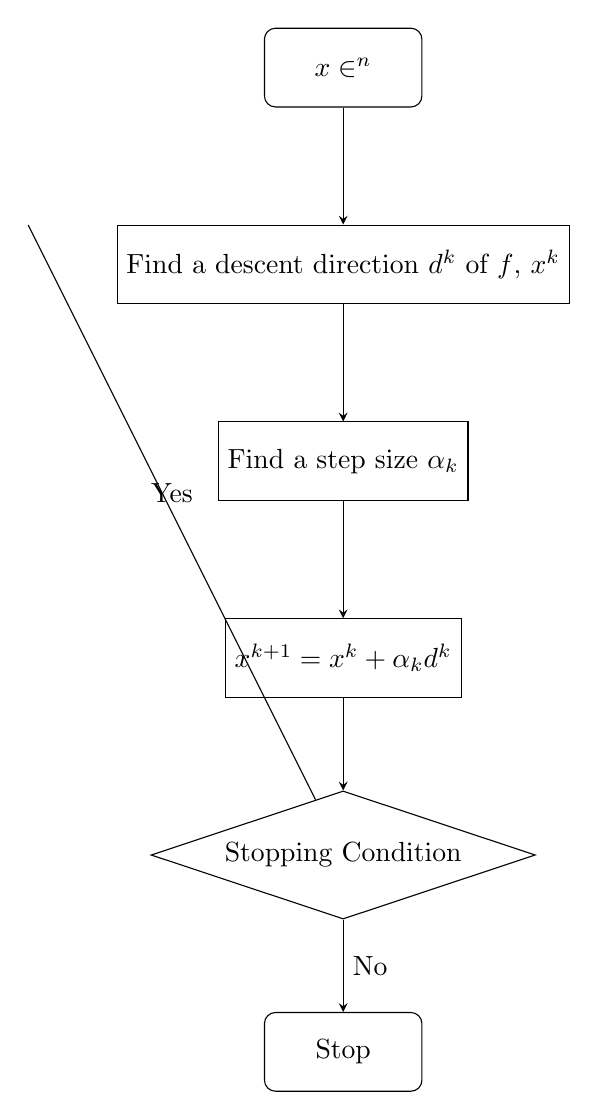
\begin{tikzpicture}[node distance=2cm]
    \node[startstop](start){$x \in \RR^n$};
    % \node[io, below of = start, yshift = -0.5cm](in1){Input};
    \node[process, below of = start, yshift = -0.5cm](pro1){Find a descent direction $d^k$ of $f$, $x^k$};
    \node[process, below of = pro1, yshift = -0.5cm](pro2){Find a step size $\alpha_k$};
    \node[process, below of = pro2, yshift = -0.5cm](pro3){$x^{k+1} = x^{k} + \alpha_k d^k$};
    \node[decision, below of = pro3, yshift = -0.5cm](dec1){Stopping Condition};
    \node[startstop, below of = dec1, yshift = -0.5cm](stop){Stop};
    % \node[process, below of = dec1, yshift = -1cm](pro2){Process 2};
    % \node[io, below of = pro2, yshift = -1cm](out1){Output};
    \coordinate (point1) at (-4cm, -2cm);
    \draw [arrow] (start) -- (pro1);
    \draw [arrow] (pro1) -- (pro2);
    \draw [arrow] (pro2) -- (pro3);
    \draw [arrow] (pro3) -- (dec1);
    \draw (dec1) -- node [above] {Yes} (point1);
    % \draw [arrow] (point1) |- (pro1);
    \draw [arrow] (dec1) -- node [right] {No} (stop);
    % \draw [arrow] (pro2) -- (out1);
    % \draw [arrow] (out1) -- (stop);
\end{tikzpicture}

\begin{enumerate}
    \item Descent Direction: For $f: \ \RR^n \rightarrow \RR$, d is a descent direction at $x$ \begin{align*}
        f^1 (x;d)=\nabla f(x)^\top d < 0
    \end{align*}
    How about steepest descent direction? With $d \in \RR^n$, \begin{align*}
        \min \ & \nabla f(x)^\top d
        \st \ & \| d \| =1
    \end{align*}
    Cauchy-Schwartz: \begin{align*}
        \nabla f^\top (x) d = \| \nabla f(x) \| \cdot \| d \| \cdot \cos \alpha
    \end{align*}
    
\end{enumerate}

\subsection{Steepest Descent Method for Minimize function}
\begin{itemize}
    \item Step 0: Start with $x^0 \in \RR^n$, pick $\varepsilon > 0$ small.
    \item Step $k$: \begin{align*}
        x^{k+1}=x^{k}- \alpha_{k} \nabla f \left(x^{k}\right)
    \end{align*}
    where \begin{align*}
        \alpha_k = \arg \min \ & f(x^k -\alpha \nabla f(x^k)) \\
        \st \ & \alpha \geq 0
    \end{align*}
    If $\| \nabla f(x^{k+1})\|<\varepsilon$, stop. Else $k \leftarrow k+1$
\end{itemize}

\begin{example}
    $\min f(x)=4 x_{1}^{2}-4 x_{1} x_{2}+2 x_{2}^{2}$\\
    $x^0=\left[\begin{array}{c}2 \\ 3\end{array}\right]$\\
    $\nabla f(x)=\left[\begin{array}{c}8 x_{1}-4 x_{2} \\ 4 x_{1}+4 x_{2}\end{array}\right]$
    $x^1 = x^0 - \alpha_0 \nabla f(x^0)$, where $\alpha_0$ solves \begin{align*}
        \min f(x^0 - \alpha \nabla f(x^0)) = \min \theta(x)
    \end{align*}
    \begin{align*}
        \theta^1 (\alpha) &= \nabla f(x^0 - \alpha \nabla f(x^0))^\top \nabla f(x^0) \\
        &= -\nabla f(2-4\alpha, 3-4\alpha)^\top \left(\begin{array}{c}4 \\ 4\end{array}\right) \\
        &= -16 (2-4\alpha) = 0 \\
        &\Rightarrow \bar{\alpha} = \frac{1}{2} \\
        \theta^2 (\alpha) &= 64 > 0
    \end{align*}
    $\therefore$ $\theta$ is convex, $\bar{\alpha} = \frac{1}{2}$ is minimizer. Then, $x^{1}=\left(\begin{array}{l}2 \\ 3\end{array}\right)-\frac{1}{2}\left(\begin{array}{l}4 \\ 4\end{array}\right)=\left(\begin{array}{l}0 \\ 1\end{array}\right)$\\
    $f\left(\begin{array}{l}2 \\ 3\end{array}\right)=10$, $f\left(\begin{array}{l}0 \\ 1\end{array}\right)=2$ \\
    $\nabla f(x^1)=\left(\begin{array}{l}-4 \\ 4\end{array}\right)$\\
    $\nabla f(x^2)^\top \nabla f(x^1)=0$ \begin{align*}
        \theta(\alpha) &= f(0-4\alpha;1-4\alpha) \\
        \theta^\prime (\alpha) &= -16(2-20\alpha)=0 \\
        &\Rightarrow \alpha_1 = \frac{1}{10} \\
        x^2 &= \left(\begin{array}{l}0 \\ 1\end{array}\right) - \frac{1}{10} \left(\begin{array}{l} -4 \\ 4\end{array}\right) = \left(\begin{array}{l}\frac{2}{5} \\ \frac{2}{5}\end{array}\right) \\
        f\left(\begin{array}{l}\frac{2}{5} \\ \frac{2}{5}\end{array}\right) &= \frac{2}{5}
    \end{align*}
\end{example}

\begin{figure}[H]
    \centering
    \includegraphics[width=5cm]{images/10-ex-1.png}
    \caption{Zigzagging}
\end{figure}

\newpage
\section{Week 12 Lecture}
\subsection{Newton's Method for Solving a System of Nonlinear Equations}
Let $H:\RR \rightarrow \RR$ be a differentiable function. Say we want to solve $h(x)=0$, with Newton's Method:\begin{align*}
    x^{k+1} = x^k - \frac{h(x^k)}{h^\prime(x^k)}
\end{align*}

\begin{figure}
    \centering
    \includegraphics[width = 7cm]{images/13-ex-1.png}
    \caption{}
\end{figure}

The equation of the target line at $(x^k, h(x^k))$ is \begin{align*}
    y = h(x^k) + h^\prime(x^k)(x - x^k)
\end{align*}
Next iterate is given by \begin{align*}
    &(y,x) = (0,x^{k+1});\\
    &-h\left(x^{k}\right)=h^{\prime}\left(x^{k}\right)\left(x^{k-1}-x^{k}\right)
\end{align*}

More generally, for a differentiable function \begin{align*}
    g=(g_1, g_2, \cdots, g_n):\RR^n \rightarrow \RR^n
\end{align*}
Newton's iterations satisfy \begin{align*}
    -g\left(x^{k}\right)=\nabla g\left(x^{k}\right)\left(x^{k-1}-x^{k}\right)
\end{align*}
or \begin{align*}
    x^{k+1}=x^{k}-\left[\nabla g(x^{k})\right]^{-1} g(x^{k}),
\end{align*}
where $\nabla g$ is the Jacobian matrix of $g$ at $x$. It is an $n \times n$ matrix where the $(i,j)$th entry is $\frac{\partial g_i(x)}{\partial x_j}$.

\subsection{Using Newton's Method to Minimize a Convex function}
$\bar{x}$ minimizes convex $f$ if \begin{align*}
    \nabla f(\bar{x}) = 0 && (\star)
\end{align*}
Apply Newton's Method to solve $(\star)$. At iteration $k$,\begin{align*}
    -\nabla f\left(x^{k}\right)= \nabla^{2} f\left(x^{k}\right)\left(x^{k+1}-x^{k}\right)
\end{align*}
or \begin{align*}
    x^{k+1}=x^{k}-\left[\nabla^{2} f\left(x^{k}\right)\right]^{-1} \nabla f\left(x^{k}\right).
\end{align*}

\begin{example}
    Use Newton's Method to minimize \begin{align*}
        f\left(x_{1}, x_{1}\right)=x_{1}^{4}+2 x_{1}^{2} x_{2}^{2}+x_{2}^{4}.
    \end{align*}
    Clearly $\bar{x}=0$ is the minimizer $a$: $f(x) \geq 0$. Start $x=(a,a)$: \begin{align*}
        -\nabla f\left(x\right) &= \nabla^{2} f\left(x\right)\left(x^{k+1}-x^{k}\right) \\
        \nabla f(x) &= \left[\begin{array}{l}
            4 x_{1}^{3}+4 x_{1} x_{2}^{2} \\
            4 x_{2}^{3}+4 x_{1}^{2} x_{2}
            \end{array}\right] \\
        \nabla^2 f(x) &= \left[\begin{array}{ll}
            12 x_{1}^{2}+4 x_{n}^{2} & 8 x_{1} x_{2} \\
            8 x_{1} x_{2} & 4 x_{1}^{2}+12 x_{2}^{2}
            \end{array}\right] \\
        -\nabla f\left(\begin{array}{l}
            a \\
            a
            \end{array}\right) &= \nabla^2 f\left(\begin{array}{l}
            a \\
            a
            \end{array}\right)\left(\begin{array}{l}
            x_{1} - a \\
            x_{2} - a
            \end{array}\right) \\
            \left[\begin{array}{c}
                8 a^{3} \\
                8 a^{3}
                \end{array}\right] &= \left[\begin{array}{cc}
                16 a^{2} & 8 a^{2} \\
                8 a^{2} & 16 a^{2}
                \end{array}\right]\left[\begin{array}{c}
                x_{1}-a \\
                x_{2} - a
                \end{array}\right]
    \end{align*}
    $\therefore$ \begin{align*}
        \left[\begin{array}{l}
            x_{1} \\
            x_{2}
            \end{array}\right]=\left[\begin{array}{l}
            2a / 3 \\
            2a / 3
            \end{array}\right]
    \end{align*}
    Thus $x^k = \left[ (\frac{2}{3})^ka, (\frac{2}{3})^ka \right]$, $k \geq 0$.
\end{example}

Questions:\begin{enumerate}
    \item Is $-\left[\nabla^{2} f\left(x^{k}\right)\right]^{-1} \nabla f\left(x^{k}\right)$ descent direction?
    \item Is $f(x^{k+1}) < f(x^k)$?
\end{enumerate}

Answers:\begin{enumerate}
    \item \begin{proof}
        If $\nabla^{2} f(x^{k})$ is positive definite and $\nabla f\left(x^{k}\right) \neq 0$, then \begin{align*}
            d = -\left[\nabla^{2} f\left(x^{k}\right)\right]^{-1} \nabla f\left(x^{k}\right)
        \end{align*}
        is a descent direction: \begin{align*}
            -\nabla f\left(x^{k}\right)\left[\nabla^{2} f\left(x^{k}\right)\right]^{-1} \nabla f\left(x^{k}\right) < 0
        \end{align*}
    \end{proof}
    \item Newton's Method may not converge to any point, let alone local minimizer!
    \begin{example}
        With $f(x)=\frac{2}{3}|x|^{3 / 2}$, start at $x^2=1$.\begin{align*}
            f^{\prime}(x)&=\left\{\begin{array}{ll}
                x^{1/ 2} & x \geq 0 \\
                (-x)^{1/2} & x<0
                \end{array}\right. \\
            f^{\prime \prime}(x)&=\left\{\begin{array}{ll}
                \frac{1}{2} x^{-1 / 2} & x \geq 0 \\
                -\frac{1}{2} x^{-1 / 2} & x<0
                \end{array}\right.
        \end{align*}
        \begin{align*}
            x^{1} &= x^{0}-2 x^{1 / 2} x^{1 / 2}=-x^{0} \\
            x^{2} &= x^{\prime}-\left(-2\left(x^{1}\right)^{1 / 2}\left(x^{\prime}\right)^{(x)}\right)=-x^{\prime}
        \end{align*}
        Then \begin{align*}
            x^k = (-1)^k, \ \forall k
        \end{align*}
        Method does not converge!
    \end{example}
\end{enumerate}

Advantage:\begin{itemize}
    \item If it converges, it converges fast!
\end{itemize}

Disadvantage:\begin{itemize}
    \item It may not converge at all.
    \item $\nabla^{2} f\left(x^{k}\right)$ may not be positive definite.
    \item Computational were complex than first-order methods.
\end{itemize}

\subsection{Interior Point Method for Linear Programming}




\end{document}